\documentclass[english,graybox,envcountchap,envcountsame,sectrefs,shortlabels]{svmono}
\usepackage{ifthen}
\newboolean{corrige}



\usepackage[T1]{fontenc}
\usepackage[latin9]{inputenc}
\usepackage[Lenny]{fncychap}
\usepackage{color}
\definecolor{page_backgroundcolor}{rgb}{1, 1, 1}
\pagecolor{page_backgroundcolor}
\definecolor{document_fontcolor}{rgb}{0, 0, 0}
\color{document_fontcolor}
\definecolor{shadecolor}{rgb}{1, 0, 0}
\usepackage{babel}
\usepackage{refstyle}
\usepackage{fancybox}
\usepackage{calc}
\usepackage{framed}
\usepackage{enumitem}
\usepackage{algorithm2e}
\usepackage{breakcites}

\usepackage{amsfonts, dsfont}
\usepackage{amsmath}
\let\proof\relax\let\endproof\relax
\usepackage{amsthm}
\usepackage{amssymb}
\usepackage{multicol,pdfsync}
\usepackage{makeidx}
\usepackage{minitoc}
\usepackage{xargs}
\usepackage{tikz}
\usetikzlibrary{positioning}
\usepackage{hyperref}
\usetikzlibrary{automata}
\usetikzlibrary{patterns}

\makeindex
\usepackage{graphicx}
%\usepackage[unicode=true,
% bookmarks=false,
% breaklinks=false,pdfborder={0 0 1},backref=section,colorlinks=false]
% {hyperref}

\makeatletter



\newtheoremstyle{style}
  {6pt}% space above
  {30pt}% space below
  {\sffamily}%body font
  {-1em}%indent amount
  {\bfseries}%Theorem head
  {}%punctuation
  {1.5em}%space after theorem head
  {}

\theoremstyle{style}
\newtheorem{exo}{\textsc{Exercise}}

\newenvironment{answer}{\noindent \\ \textbf{Solution.}\begin{leftbar} \footnotesize}{\hfill \qed \end{leftbar}}

%\newtheoremstyle{styleQuestion}
%  {6pt}% space above
%  {6pt}% space below
%  {\sffamily}%body font
%  {13.5pt}%indent amount
%  {\sffamily}%Theorem head
%  {.}%punctuation
%  {0.5em}%space after theorem head
%  {}
%
%\ifthenelse{\boolean{corrige}}%
% {\theoremstyle{styleQuestion}%
% \newtheorem{question}{}}%
% {\theoremstyle{styleQuestion}%
% \newtheorem{question}{}}

\ifthenelse{\boolean{corrige}}%
   {}
   {\usepackage{environ}
   \NewEnviron{hide}{}
   \let\answer\hide
   \let\endanswer\endhide}

%%%%%%%%%%%%%%%%%%%%%%%%%%%%%% LyX specific LaTeX commands.

\AtBeginDocument{\providecommand\Eqref[1]{\ref{Eq:#1}}}
\AtBeginDocument{\renewcommand\eqref[1]{(\ref{#1})}}
\AtBeginDocument{\providecommand\Defref[1]{\ref{def:#1}}}
\AtBeginDocument{\providecommand\defref[1]{\ref{def:#1}}}
\AtBeginDocument{\providecommand\Lemref[1]{\ref{Lem:#1}}}
\AtBeginDocument{\providecommand\algref[1]{\ref{alg:#1}}}
\AtBeginDocument{\providecommand\Propref[1]{\ref{Prop:#1}}}
\AtBeginDocument{\providecommand\Thmref[1]{\ref{Thm:#1}}}
\AtBeginDocument{\providecommand\thmref[1]{\ref{thm:#1}}}
\AtBeginDocument{\providecommand\Corref[1]{\ref{Cor:#1}}}
\AtBeginDocument{\providecommand\Subsecref[1]{\ref{Subsec:#1}}}

\RS@ifundefined{subsecref}
  {\newref{subsec}{name = \RSsectxt}}
  {}
\RS@ifundefined{thmref}
  {\def\RSthmtxt{theorem~}\newref{thm}{name = \RSthmtxt}}
  {}
\RS@ifundefined{lemref}
  {\def\RSlemtxt{lemma~}\newref{lem}{name = \RSlemtxt}}
  {}

\newcounter{hypH}
\newenvironment{hypH}{
    \refstepcounter{hypH}
    \begin{itemize}
    \item[{\bf H\arabic{hypH}}]
    }
{\end{itemize}}


%%%%%%%%%%%%%%%%%%%%%%%%%%%%%% Textclass specific LaTeX commands.
\newenvironment{svmultproof}{\small \begin{proof}}{\end{proof}}
\renewenvironment{keywords}{\textit{\bf Keywords: } \sffamily }{}

%%%%%%%%%%%%%%%%%%%%%%%%%%%%%% User specified LaTeX commands.
\usepackage{a4wide,appendix,wrapfig}
\usepackage{bbm}
\definecolor{shadecolor}{RGB}{211,211,211}
\usepackage{pgf,framed}
%\renewenvironment{proof}%
%{\noindent \small {\textsc{Proof}.} \footnotesize}%
%{ \hfill$\blacksquare$\\}

\newenvironment{hyp}[1]{
\begin{enumerate}[label=(\textbf{\sf #1}\arabic*),resume=hyp#1]\begin{sf}}
{\end{sf}\end{enumerate}}



\global\long\def\defref#1{Definition~\ref{def:#1}}
\global\long\def\Defref#1{Definition~\ref{def:#1}}
\global\long\def\Lemref#1{Lemma~\ref{lem:#1}}
\global\long\def\Propref#1{Proposition~\ref{prop:#1}}
\global\long\def\Eqref#1{(\ref{eq:#1})}
\global\long\def\Thmref#1{Theorem~\ref{thm:#1}}
\global\long\def\lemref#1{Lemma~\ref{lem:#1}}
\global\long\def\propref#1{Proposition~\ref{prop:#1}}
\global\long\def\thmref#1{Theorem~\ref{thm:#1}}
\global\long\def\Subsecref#1{Section~\ref{subsec:#1}}
\global\long\def\Corref#1{Corollary~\ref{cor:#1}}
\global\long\def\algref#1{Algorithm~\ref{alg:#1}}


\newcommand{\iid}{\stackrel{\mathrm{i.i.d}}{\sim}}
\newcommandx{\dens}[3][1=,2=]%
{
\operatorname{p}_{#1}^{#2}(#3)
}
\newcommandx{\aslim}[1]{\ensuremath{\stackrel{#1 \mbox{-} \text{a.s.}}{\longrightarrow}}}
\newcommand{\Zset}{\mathsf{Z}}
\newcommand{\Zsigma}{\mathcal{Z}}
\newcommand{\borel}{\mathcal{B}}
\newcommand{\weaklim}{\ensuremath{\stackrel{\mathcal{L}_{\PP}}{\Rightarrow}}}
\newcommand{\eqLaw}{\stackrel{\mathcal L}{=}}
\newcommand{\indep}{\rotatebox[origin=c]{90}{$\models$}}
\newcommandx\functionsetspec[1][1=]{
\ifthenelse{\equal{#1}{c}}{\mathrm{C}}%fonctions continues
{\ifthenelse{\equal{#1}{bc}}{\mathrm{C}_b}%fonctions continues born\'{e}es
{\ifthenelse{\equal{#1}{u}}{\mathrm{U}}%fonctions uniform\'{e}ment continues
{\ifthenelse{\equal{#1}{bu}}{\mathrm{U}_b}%fonctions uniform\'{e}ment continues born\'{e}es
{\ifthenelse{\equal{#1}{l}}{\mathrm{Lip}}%fonctions lipschitz
{\ifthenelse{\equal{#1}{bl}}{\mathrm{Lip}_b}%fonctions lipschitz born\'{e}es
{\mathbb{F}_{#1}}%le reste
}}}}}}
\newcommandx\sequence[3][2=,3=]
{\ifthenelse{\equal{#3}{}}{\ensuremath{\{ #1_{#2}\}}}{\ensuremath{\{ #1_{#2}, \eqsp #2 \in #3 \}}}}
\newcommand{\Yset}{\mathsf{Y}}
\newcommand{\Ysigma}{\mathcal{Y}}
\newcommandx\dsequence[4][3=,4=]{\ensuremath{\{ (#1_{#3}, #2_{#3}), \eqsp #3 \in #4 \}}}
\newcommand{\Id}{\mathrm{I}}
\newcommand{\lrav}[1]{\left|#1 \right|}
\newcommand{\rme}{\mathrm{e}}
\newcommand{\rmi}{\mathrm{i}}
\newcommand{\fracc}[2]{\frac{#1}{#2}}
\newcommand{\bs}{\begin{shaded}}
\newcommand{\es}{\end{shaded}}
\newcommand{\bfr}{\begin{framed}}
\newcommand{\efr}{\end{framed}}
\newcommand{\blb}{\begin{leftbar}}
\newcommand{\elb}{\end{leftbar}}
\newcommand{\ltwo}{\mathrm{L}_2}
\newcommand{\dlim}[1]{\stackrel{\mathcal{L}_{#1}}{\Rightarrow}}
\newcommand{\plim}[1]{\stackrel{#1-prob}{\longrightarrow}}
\newcommand{\gauss}{\mathcal{N}}
\newcommand{\eqsp}{}
\newcommand{\xset}{\ensuremath{\mathsf{X}}}
\newcommand{\Xset}{\mathsf{X}}
\newcommand{\Xsigma}{\mathcal{X}}


\newcommand{\Uset}{\mathsf{U}}
\newcommand{\Usigma}{\mathcal{U}}
\makeatother

\providecommand{\corollaryname}{Corollary}
\providecommand{\definitionname}{Definition}
\providecommand{\examplename}{Example}
\providecommand{\exercisename}{Exercise}
\providecommand{\lemmaname}{Lemma}
\providecommand{\proofname}{Proof}
\providecommand{\propositionname}{Proposition}
\providecommand{\theoremname}{Theorem}

\begin{document}
\global\long\def\1{\mathbf{1}}%
\global\long\def\as{\PP-\mbox{a.s.}}%
\global\long\def\eqdef{:=}%
\global\long\def\eqlaw{\stackrel{\mathcal{L}}{=}}%
\global\long\def\funcset#1{\mathsf{F_{#1}}}%
\global\long\def\indi#1{\1_{#1}}%
\global\long\def\indiacc#1{\indi{\left\{  #1\right\}  }}%
\global\long\def\lfuncset#1{\mathsf{L_{#1}}}%
\global\long\def\lr#1{\left(#1\right)}%
\global\long\def\PE{\mathbb{E}}%
\global\long\def\lrb#1{\left[#1\right]}%
\global\long\def\lrcb#1{\left\{  #1\right\}  }%
\global\long\def\mcbb{\mathcal{B}}%
\global\long\def\meas#1{\mathsf{M}_{#1}}%
\global\long\def\mh#1{P_{\langle#1\rangle}^{MH}}%
\global\long\def\nset{\mathbb{N}}%
\global\long\def\mc#1{\mathcal{#1}}%
\global\long\def\mcf{\mathcal{F}}%
\global\long\def\mcg{\mathcal{G}}%
\global\long\def\PP{\mathbb{P}}%
\global\long\def\rmd{\mathrm{d}}%
\global\long\def\rset{\mathbb{R}}%
\global\long\def\seq#1#2{\lrcb{#1\,:\,#2}}%
\global\long\def\set#1#2{\lrcb{#1\,:\,#2}}%
\global\long\def\Xset{\mathsf{X}}%
\global\long\def\Xsigma{\mathcal{X}}%




\title{Introduction to computational statistics}
\author{Sylvain Le Corff}
%\subtitle{A crash course Monte Carlo methods for generative models
%\begin{figure}[!h]
%\centering
%\includegraphics[height=80pt]{hamilton.jpg}
%\includegraphics[height=80pt]{bayes.jpg}
%\includegraphics[height=80pt]{markov.jpg}
%\includegraphics[height=80pt]{ulam.jpg}
%\includegraphics[height=80pt]{metropolis.png}
%\includegraphics[height=80pt]{hastings.jpg}
%\end{figure}
%}
\date{}

\maketitle

\tableofcontents

\chapter{Markov chain Monte Carlo}

\section{Introduction}
This chapter aims at designing algorithms to obtain samples from a complex distribution $\pi$ defined on a measurable space $(\mathsf{X},\mathcal{X})$. Such algorithms can be applied in many situations, and the target distribution can have several forms depending on the different contexts. In many areas of statistics and machine learning, we are interested in drawing samples from $\pi$ although $\pi$ is known only up to a normalizing constant. Such situations arise naturally in a wide variety of contexts, for example, in Bayesian inference, where $\pi$ represents a posterior distribution over parameters given data, or in energy-based models, where $\pi$ is a probability distribution defined through an energy function.

Direct sampling from $\pi$ is often infeasible, either because the distribution has a complex, high-dimensional structure or because computing the normalizing constant is intractable. Markov Chain Monte Carlo (MCMC) methods provide a powerful framework for addressing this challenge. The central idea is to construct a Markov chain whose stationary distribution is precisely $\pi$, and then to use the long-run behavior of the chain to generate approximate samples from $\pi$.

%The target distribution can be given for instance by a marginal density $p_\theta(y) = \int p_\theta(x,y) \lambda(\rmd x)$ or by a conditional/posterior distribution $p_\theta(x|y) = p_\theta(x)p_\theta(y|x)/\int p_\theta(x,y) \lambda(\rmd x)$ where $\theta\in\Theta$ and $\lambda$ is a dominating measure.

%For instance, in the previous chapters, the E-step of the EM algorithm requires to compute en expectation under the probability density $z \mapsto p_\theta(z|X)$ which is not possible exactly in almost all settings. The intermediate quantity  can therefore be replaced by a Monte Carlo  estimator by sampling random variables with distribution $p_\theta(z|X)\propto p_\theta(z)p_\theta(X|z)$. We aim at sampling from a probability distribution that we only know up to a multiplicative constant.

 %In this section, we introduce different algorithms, depending on the framework, to solve machine learning tasks based on sampling random variables.  In particular, we detail Markov Chain Monte Carlo (MCMC) methods, which allow to construct a process $(X_k)_{k\in\nset}$ that targets an unknown distribution $\pi$. Sometimes $(X_k)_{k\in\nset}$ is itself a Markov chain with invariant probatility measure $\pi$, sometimes, $(X_k)_{k\in\nset}$ is the first component process of an extended Markov chain that targets an extended distribution where the marginal distribution on the first component is $\pi$.

%\begin{example}
%%\paragraph{Bayesian inference. }
%In  Bayesian inference, prior belief  is combined with
%data to obtain posterior distributions on which statistical inference is based.
%%Although we focus primarily on  likelihood based inference in this text,
%%it is also worthwhile to consider Bayesian  inference  for some problems.
%Except for some simple cases, Bayesian inference can be computationally
%intensive and may rely on  computational techniques.
%
%
%The basic idea in Bayesian analysis is that a parameter vector $ \theta \in \Theta$ is unknown, so it is endowed with a \emph{prior} distribution with probability density
%$\pi_0( \theta)$.  We also
%introduce a model or likelihood, $\dens[][]{ y_{1:n} \mid \theta}$, that is
%a probability density function for the data $y_{1:n}$ which depends on the parameter vector.
%Inference about $ \theta$ is then based on the \emph{posterior}
%distribution, which is obtained via Bayes's theorem,
%$$
%\theta \mapsto \pi(\theta) =\frac{\pi_0( \theta) \dens[][]{ y_{1:n} \mid \theta}}{\int \pi_0( \theta) \dens[][]{ y_{1:n} \mid \theta} \lambda(\rmd \theta)} \propto \pi_0( \theta) \dens[][]{ y_{1:n} \mid \theta}.
%$$
%  In some simple cases, the prior  and
%the likelihood are \emph{conjugate}  distributions that may be combined easily.
%For example, in $n$ fixed repeated (i.i.d.) Bernoulli experiments with probability of success $\theta$,
%a \emph{Beta-Binomial} conjugate pair is taken.  In this case the prior is
%Beta($a,b$):
%$\pi_0(\theta) \propto \theta^{a} (1-\theta)^{b}\mathds{1}_{(0,1)}(\theta)$; the values $a,b > -1$  are called
%hyperparameters. The likelihood in this example is
%Binomial$(n,\theta)$:
%$\dens[][]{ y \mid \theta} \propto \theta^y (1-\theta)^{n-y}$, from which
%we easily deduce that the
%posterior is also Beta,
%$\pi ( \theta ) \propto \theta^{y+a}(1-\theta)^{n+b-y }\mathds{1}_{(0,1)}(\theta)
%$, and from which inference may easily be achieved.
%
%In more complex experiments, the posterior distribution is often difficult to obtain by direct calculation,
%so alternatives have to be deployed to obtain samples approximately distributed as the posterior distribution. 
%\end{example}
%%Note that in \eqref{eq:target:bayes}, the numerator is usually known and explicit while, due to the integral, the denominator is a multiplicative unknown constant.  

\begin{example}
Energy-based models (EBM) are very flexible models which describe the target distribution using an unnormalized function, referred to as the energy function. These models are easier to design that models with a tractable likelihood such as autoregressive models, in particular in high-dimensional setting. As the energy function is not normalized, it can
be easily parameterized with any nonlinear regression function. Using neural networks such as Multi-layer Perceptrons, or convolutional neural networks,  it is straightforward to introduce energy function with specific structures depending nonlinearly on the input. %We can choose specific
%architectures tailored for every type of data, see \cite{song2021train} for a recent overview of EBM.

In a generic setting, the target random variable takes values in $(\rset^d,\mathcal{B}(\rset^d))$ and the target distribution (the target density with respect to the Lebesgue measure) is written:
$$
x\mapsto \pi_\theta(x) \propto \exp\left(-\mathrm{E}_\theta(x)\right) = \frac{\exp\left(-\mathrm{E}_\theta(x)\right)}{\int \exp\left(-\mathrm{E}_\theta(u)\right)\rmd u},
$$
where $\theta$ is an unknown parameter to estimate and $\mathrm{E}_\theta$ is the energy function. The normalizing constant is often written $Z_\theta$ and referred to as the partition function:
$$
Z_\theta = \int \exp\left(-\mathrm{E}_\theta(u)\right)\rmd u.
$$
Since $Z_\theta$ is an intractable integral, evaluation and
differentiation of $x\mapsto \log \pi_\theta(x)$ is not possible in usual settings. In order to estimate the unknwon parameter $\theta$ using i.i.d. data, an appealing approach is to use gradient-based maximization procedures of the likelihood function. This means that we need to compute:
$$
x\mapsto \nabla_\theta \log\pi_\theta(x) = -\nabla_\theta\mathrm{E}_\theta(x) - \nabla_\theta \log Z_\theta.
$$
The first term can be evaluated easily as $\mathrm{E}_\theta(x)$ is known. For the second term, we can write, under regularity assumptions on the model:
\begin{multline*}
\nabla_\theta \log Z_\theta = Z_\theta^{-1} \int \nabla_\theta\exp\left(-\mathrm{E}_\theta(u)\right)\rmd u \\=  \int \left\{-\nabla_\theta \mathrm{E}_\theta(u)\right\}Z_\theta^{-1}\exp\left(-\mathrm{E}_\theta(u)\right)\rmd u = \int \left\{-\nabla_\theta \mathrm{E}_\theta(u)\right\}\pi_\theta(u)\rmd u .
\end{multline*}
Therefore $\nabla_\theta \log Z_\theta = \mathbb{E}_{\pi_\theta}[-\nabla_\theta \mathrm{E}_\theta(X)]$ where $\mathbb{E}_{\mu}[f(X)]$ denotes the expectation of $f(X)$ when $X\sim \mu$. Therefore, it is possible to train an EBM by providing a Monte Carlo estimate of $\nabla_\theta \log Z_\theta$ which requires to obtain samples from $\pi_\theta$. However, this is not straightforward as $\pi_\theta$ is known only up to a multiplicative normalizing constant (as in the Bayesian setting).
\end{example}

%\begin{example}
%In Bayesian deep learning, uncertainty quantification may be obtained by analyzing the posterior distribution of the weights, as in \cite{blundell2015weight}. In this setting, using an input $x\in \rset^p$, the observations $Y$, conditionally on the parameter $\theta$, has a Gaussian distribution with mean $m_\theta(x)$ and covariance $\Sigma_\theta(x)$. The quantities  $m_\theta(x)$ and  $\Sigma_\theta(x)$ are outputs of a neural network (for instance a Multi-layer Perceptron) with input $x$ and parameters $\theta$. The prior distribution of $\theta$ is Gaussian with independent entries with mean $\mu \in\rset$ and varriance $\sigma^2>0$. Since $m_\theta(x)$ and  $\Sigma_\theta(x)$ contain many nonlinearities the posterior distribution $\pi$ of $\theta$, i.e. the distribution of $\theta$ given $Y$ and the input $x$, is unknown.


\section{Key elements on Markov chains}
Let $(\Xset,\Xsigma)$ be a measurable space, i.e.  $\Xsigma$ is a $\sigma$-algebra on $\Xset$, and consider the following notations.
\begin{itemize}[-]
\item $\meas +(\Xset)$ is the set of non-negative measures on $(\Xset,\Xsigma)$.
\item $\meas 1(\Xset)$ is the set of probability measures on $(\Xset,\Xsigma)$.
\item $\funcset{}(\Xset)$ is the set of real-valued measurable functions
$f$ on $\Xset$ and $\funcset{}_{+}(\Xset)$ the set of non-negative measurable
functions on $\Xset$.
\item If $k\leq\ell$, $(u_{k},\ldots,u_{\ell})$ is denoted by $u_{k:\ell}$   and $(u_{k+\ell})_{\ell\in\nset}$ by $u_{k:\infty}$.
\end{itemize}

\begin{definition}
We say that $P:\Xset\times\Xsigma\to\rset^{+}$
is a Markov kernel if, for all $(x,A)\in\Xset\times\Xsigma$,
\begin{itemize}[-]
\item $\Xset\ni y\mapsto P(y,A)$ is $\Xsigma/\mcbb(\rset^{+})$ measurable,
\item $\Xsigma\ni B\mapsto P(x,B)$ is a probability measure on $(\Xset,\Xsigma)$.
\end{itemize}
\end{definition}
For all $(x,A)\in\Xset\times\Xsigma$, as a function
of the first component only, $P(\cdot,A)$ is measurable and as a
function of the second component only, $P(x,\cdot)$ is a probability
measure. In particular, $P(x,\Xset)=1$ for all $x\in\Xset$. Since
$P(x,\cdot)$ is a measure, we also use the infinitesimal notation:
$P(x,\rmd y)$. For example, 
$$
P(x,A)=\int_{\Xset}\indi A(y)P(x,\rmd y)=\int_{A}P(x,\rmd y)\eqsp.
$$
%In almost all the course, a Markov kernel $P$ allows to move a point $x$ from a measurable space $(\Xset,\Xsigma)$ to another point on the same measurable space, that is, $P$ is defined on $\Xset\times \Xsigma$ but we can more generally define a Markov kernel from a measurable space $(\Xset,\Xsigma)$ to another measurable space $(\Yset,\Ysigma)$. In such case, $P$ will be a  Markov kernel on $\Xset \times \Ysigma$. 
For all $\mu\in\meas +(\Xset)$, all Markov kernels $P$, $Q$ on
$\Xset\times\Xsigma$, and all measurable non-negative or bounded
functions $h$ on $\Xset$, we use the following conventions and
notations.
\begin{itemize}[-]
\item $\mu P$ is the (positive) measure: $\Xsigma\ni A\mapsto\mu P(A)=\int\mu(\rmd x)P(x,A)$,
\item $PQ$ is the Markov kernel: $(x,A)\mapsto\int_{\Xset}P(x,\rmd y)Q(y,A)$,
\item $Ph$ is the measurable function $x\mapsto\int_{\Xset}P(x,\rmd y)h(y)$.
\end{itemize}
It is easy to check that if $\mu$ is a probability measure, then
$\mu P$ is also a probability measure (since $\mu P(\Xset)=\int_{\Xset}\mu(\rmd x)P(x,\Xset)=\int_{\Xset}\mu(\rmd x)=1$).
With this notation, using Fubini's theorem,
\begin{align*}
\mu(P(Qh)) & =(\mu P)(Qh)=(\mu(PQ))h\\
 & =\mu((PQ)h)=\int_{\Xset^{3}}\mu(\rmd x)P(x,\rmd y)Q(y,\rmd z)h(z).
\end{align*}
%Therefore, all these parenthesis can be discarded and we can write
%$\mu PQh$ without any ambiguity. 
%To sum up, measures act on the left side of a Markov kernel whereas
%functions acts on the right side. To make sure you have mastered all
%the notation, check your understanding with the following equalities
%$\delta_{x}P(A)=P(x,A)=P\indi A(x)$.
For a given
Markov kernel $P$ on $\Xset\times\Xsigma$, define $P^{0}=\mathrm{Id}$ where
$\mathrm{Id}$ is the identity kernel: $(x,A)\mapsto\indi A(x)$, and set for
$k\geq0$, $P^{k+1}=P^{k}P$.


\begin{definition}
Let $\seq{X_{k}}{k\in\nset}$
be a sequence of random variables on the same probability space $(\Omega,\mcg,\PP)$
and taking values on $\Xset$, we say that $\seq{X_{k}}{k\in\nset}$
is a Markov chain with Markov kernel $P$ and initial distribution
$\nu\in\meas 1(\Xset)$ if and only if the two following statements hold.
\begin{enumerate}[i)]
\item  For all $(k,A)\in\nset\times\Xsigma$,  $\PP(X_{k+1}\in A|X_{0:k})=P(X_{k},A)$,
$\PP$-a.s.
\item $\PP(X_{0}\in A)=\nu(A)$.
\end{enumerate}
\end{definition}
Note that, in this definition, we consider $\PP(X_{k+1}\in A|X_{0:k})$,
that is, the conditional probability is with respect to the sigma-field
$\sigma(X_{0:k})$. We can replace $\sigma(X_{0:k})$ by
$\mcf_{k}$ as soon as we know that $(X_{k})_{k\geq0}$ is $(\mcf_{k})_{k\geq0}$-adapted.

\begin{definition}
We say that $\pi\in\meas 1(\Xset)$ is an invariant probability measure
for the Markov kernel $P$ on $\Xset\times\Xsigma$ if $\pi P=\pi$.
\end{definition}
If $(X_{k})$ is a Markov chain with Markov kernel $P$
and assuming that $X_{0}\sim\pi$, then for all $k\geq1$, we have
$X_{k}\sim\pi$ since $\pi P^{k+1}=\pi P^{k}$ and
therefore, for all $k\in\nset$, $\pi P^{k}=\pi$.  It can be readily checked that if $\pi$ is an \emph{invariant
probability measure }for $P$, then the sequence of random variables
$\seq{X_{k}}{k\in\nset}$ is a \emph{strongly stationary sequence} in the sense that for all $n,p\in\nset^{*}$,
and all n-tuple $k_{1:n}$, the random vector $(X_{k_{1}},\ldots,X_{k_{n}})$
has the same distribution as $(X_{k_{1}+p},\ldots,X_{k_{n}+p})$.

\begin{definition}
Let $\pi\in\meas 1(\Xset)$ and $P$ be a Markov kernel on $\Xset\times\Xsigma$.
We say that $P$ is $\pi$-reversible if and only if  for all measurable bounded or non-negative functions $h$
on $\left(\Xset^{2},\Xsigma^{\otimes2}\right)$,
\begin{equation}
\iint_{\Xset^{2}}h(x,y)\pi(\rmd x)P(x,\rmd y)=\iint_{\Xset^{2}}h(x,y)\pi(\rmd y)P(y,\rmd x).\label{eq:reversibility:h}
\end{equation}
A Markov kernel $P$ is $\pi$-reversible if and only
if the probability measure $\pi(\rmd x)P(x,\rmd y)$ is symmetric
with respect to $(x,y)$. We often write, with infinitesimal
notation,
\begin{equation}
\label{eq:reversibility}
\pi(\rmd x)P(x,\rmd y)=\pi(\rmd y)P(y,\rmd x)\eqsp.
\end{equation}
\end{definition}
\begin{proposition}
Let $P$ be a Markov kernel on $\Xset\times\Xsigma$. Let $\pi\in\meas 1(\Xset)$
such that $P$ is $\pi$-reversible, then the Markov kernel $P$ is
$\pi$-invariant.
\end{proposition}

\begin{proof}
For any $A\in\Xsigma$, 
\[
\pi P(A)=\iint_{\Xset^{2}}\indi A(y)\pi(\rmd x)P(x,\rmd y)=\iint_{\Xset^{2}}\indi A(y)\pi(\rmd y)P(y,\rmd x)=\int_{A}\pi(\rmd y)P(y,\Xset)=\pi(A),
\]
which completes the proof.
\end{proof}
Therefore, if we want to check easily that
a kernel $P$ is $\pi$-invariant, it is sufficient to check that
it is $\pi$-reversible.


\begin{figure}
\label{fig:inv:hist}
\centering
\includegraphics[scale=0.6]{hist_mh}
\caption{Histogram of a Gaussian AR($1$) process, $X_k = \mu + \phi X_{k-1} + \sigma Z_k$, where $(Z_k)_{k\in \nset}$ is an iid sequence of standard Gaussian random variables, independent of $X_0$ with $|\phi| < 1$. The Gaussian distribution with mean $\mu/(1-\phi)$ and variance $\sigma^2/(1-\phi^2)$ is a stationary distribution of the Markov chain. Illustration of the histogram  and of the stationary distribution with $\mu =1$, $\phi = 0.9$ and $\sigma = 1$.}
\end{figure}


\section{Metropolis-Hastings algorithm}
In this section, we are given a probability measure $\pi\in\meas 1(\Xset)$
and the idea now is to construct a Markov chain $\seq{X_{k}}{k\in\nset}$
admitting $\pi$ as invariant probability measure, in which case we
say that $\pi$ is a target distribution. In other words, we try to
find a Markov kernel $P$ on $\Xset\times\Xsigma$ such that $P$
is $\pi$-invariant. %The reason for that is that an invariant probability
%measure will be a good candidate for the ``limiting'' distribution
%of $\seq{X_{k}}{k\in\nset}$ (in some sense to be defined) and this
%in turn, will allow us to provide an approximation of $\pi(h)=\int_{\Xset}h(x)\pi(\rmd x)$ of the form $n^{-1}\sum_{k=0}^{n-1}h(X_{i})$ for any measurable function $h$. 


For simplicity we now assume that $\pi$ has a density with respect
to some dominating $\sigma$-finite measure $\mu$ and by abuse
of notation, we also denote by $\pi$ this density, that is we write
$\pi(\rmd x)=\pi(x)\mu(\rmd x)$ and we assume that this density
$\pi$ is positive. Moreover, let $Q$ be a Markov kernel on $\Xset\times\Xsigma$ such
that $Q(x,\rmd y)=q(x,y)\mu(\rmd y)$, that is, for any $x\in\Xset$,
$Q(x,\cdot)$ is also dominated by $\mu$ and denoting by $q(x,\cdot)$
this density, we assume for simplicity that $q(x,y)$ is positive
for all $x,y\in\Xset$. 

For a given function $\alpha:\Xset^{2}\to[0,1]$,  Algorithm~\ref{alg:mh} describes the Metropolis algorithm.

\begin{algorithm}
\caption{\label{alg:mh}The Metropolis Algorithm}
%\SetAlgoLined
\SetKwInOut{Input}{Input}\SetKwInOut{Output}{Output}
\Input{Initial distribution $\mu$, maximum number of iterations $n$.}
\Output{Markov chain $X_0,\ldots,X_n$.}
\BlankLine
At iteration $k=0$, draw $X_{0}\sim \mu$.\\
\For{$k = 0$ \KwTo $n-1$}
{
$\bullet$ Draw independently $Y_{k+1}\sim Q(X_{k},\cdot)$ and $U_{k+1}\sim\mathrm{U}(0,1)$.\\
$\bullet$ Set $X_{k+1}=\begin{cases} Y_{k+1} & \mbox{if }U_{k+1}\eqsp,\leq\alpha(X_{k},Y_{k+1})\\ X_{k} & \mbox{otherwise}\eqsp. \end{cases}$
}
\end{algorithm}
The Markov kernel $Q$ allows to propose a candidate for the next value of
the Markov chain $(X_{k})_{k\in\nset}$ and this candidate is accepted or
rejected according to a probability that depends on the function $\alpha$. We now choose conveniently $\alpha$ in such a way that $(X_{k})_{k\in\nset}$
is a Markov chain with invariant probability measure $\pi$. 
%To do so, let us assume that
%for all $x,y\in\Xset$,
%\begin{equation}
%\pi(x)\alpha(x,y)q(x,y)=\pi(y)\alpha(y,x)q(y,x),\label{eq:balance}
%\end{equation}
%and let us show that it implies that the Markov kernel P associated
%with $(X_{k})_{k\in\nset}$ is $\pi$-reversible.
First, we write down the Markov kernel associated with $(X_{k})_{k\in\nset}$. Write $\mcf_{k}=\sigma(X_{0},U_{1:k},Y_{1:k})$
and note that $(X_{k})_{k\in\nset}$ is adapted to the filtration $(\mcf_{k})_{k\in\nset}$
(which is equivalent to $\sigma(X_{0:k})\subset\mcf_{k}$). Then,
setting $\bar{\alpha}(x)=1-\int_{\Xset}Q(x,\rmd y)\alpha(x,y)$, we
have for any bounded or non-negative measurable function $h$ on $\Xset$
and any $k\in\nset$,
\begin{align*}
\PE\lrb{h(X_{k+1})|\mcf_{k}} & =\PE\lrb{\indiacc{U_{k+1}<\alpha(X_{k},Y_{k+1})}h(Y_{k+1})|\mcf_{t}}+\PE\lrb{\indiacc{U_{k+1}\geq\alpha(X_{k},Y_{k+1})}|\mcf_{k}}h(X_{k})\\
 & =\int_{\Xset}Q(X_{k},\rmd y)\alpha(X_{k},y)h(y)+\bar{\alpha}(X_{k})h(X_{k})\\
 & =\int_{\Xset}\lrb{Q(X_{k},\rmd y)\alpha(X_{k},y)+\bar{\alpha}(X_{k})\delta_{X_{k}}(\rmd y)}h(y)=\mh{\pi,Q}h(X_{k}).
\end{align*}
Therefore, $\seq{X_{k}}{k\in\nset}$ is a Markov chain with Markov
kernel
\begin{equation}
\mh{\pi,Q}(x,\rmd y)=Q(x,\rmd y)\alpha(x,y)+\bar{\alpha}(x)\delta_{x}(\rmd y).\label{eq:def:mh}
\end{equation}

\begin{lemma}
\label{lem:reversible} The Markov kernel $\mh{\pi,Q}$ is $\pi$-reversible
if and only if  for all measurable bounded or non-negative functions $h$
on $\left(\Xset^{2},\Xsigma^{\otimes2}\right)$,
\begin{equation}
\int_{\Xset^2} h(x,y)\pi(\rmd x)Q(x,\rmd y)\alpha(x,y)= \int_{\Xset^2} h(x,y)\pi(\rmd y)Q(y,\rmd x)\alpha(y,x).\label{eq:balance:detaillee}
\end{equation}
\end{lemma}
Equation \eqref{eq:balance:detaillee} is often called
the detailed balance condition.
\begin{proof}
First, note that
\begin{equation}
\pi(\rmd x)\bar{\alpha}(x)\delta_{x}(\rmd y)=\pi(\rmd y)\bar{\alpha}(y)\delta_{y}(\rmd x).\label{eq:balance:dirac}
\end{equation}
Indeed, for any measurable function $h$ on $\Xset^{2}$, we have
\begin{align*}
\iint_{\Xset^{2}}h(x,y)\pi(\rmd x)\bar{\alpha}(x)\delta_{x}\lr{\rmd y} & =\int_{\Xset}h(x,x)\pi(\rmd x)\bar{\alpha}(x)\\
 & =\int_{\Xset}h(y,y)\pi(\rmd y)\bar{\alpha}(y)=\iint_{\Xset^{2}}h(x,y)\pi(\rmd y)\bar{\alpha}(y)\delta_{y}(\rmd x).
\end{align*}
Combining \eqref{eq:def:mh} with \eqref{eq:balance:dirac}, we obtain that
$\mh{\pi,Q}$ is $\pi$-reversible if and only if the detailed balance
condition \eqref{eq:balance:detaillee} is satisfied. This completes
the proof.
\end{proof}

We now provide an explicit expression of the acceptance probability $\alpha$. The proof of Lemma~\ref{lem:acceptance} is straightforward.


\begin{lemma}
\label{lem:acceptance} Define 
$$
\alpha^{MH}(x,y)=\min\lr{\frac{\pi(y)q(y,x)}{\pi(x)q(x,y)},1}
$$
and 
$$
\alpha^{b}(x,y)=\frac{\pi(y)q(y,x)}{\pi(x)q(x,y)+\pi(y)q(y,x)}.
$$
Then, $\alpha^{MH}$ and $\alpha^{b}$ satisfy
the detailed balance condition \eqref{eq:balance:detaillee}. 
\end{lemma}

%\begin{proof}
%The fact that any $\alpha\in\left\{ \alpha^{MH},\alpha^{b}\right\} $
%satisfies $\pi(x)q(x,y)\alpha(x,y)=\pi(y)q(y,x)\alpha(y,x)$ for $\lambda^{\otimes2}$-almost
%all $x,y\in\Xset$, is immediate, by plugging the value of $\alpha$ in the equation.
%It remains to check \eqref{eq:accept:max}. Assume now that for $\lambda^{\otimes2}$-almost
%all $x,y\in\Xset$,
%\[
%\pi(x)q(x,y)\alpha(x,y)=\pi(y)q(y,x)\alpha(y,x).
%\]
%then, using that $\alpha(y,x)\leq1$ shows that $\alpha(x,y)\leq\frac{\pi(y)q(y,x)}{\pi(x)q(x,y)}$.
%Moreover, $\alpha(x,y)\leq1$ and this finally implies
%\[
%\alpha(x,y)\leq\min\left(\frac{\pi(y)q(y,x)}{\pi(x)q(x,y)},1\right)=\alpha^{MH}(x,y),
%\]
%which completes the proof.
%\end{proof}



\begin{example}[The random walk MH sampler]
If $\Xset=\rset^{p}$ and if
the proposal kernel is $Q(x,\rmd y)=q(y-x)\lambda(\rmd y)$ where
$q$ is a symmetric density with respect to $\lambda$ on $\Xset$, (by symmetric,
we mean that $q(u)=q(-u)$ for all $u\in\Xset$) then at each time
step in the MH algorithm, we draw a candidate $Y_{k+1}\sim q\left(y\ -X_{k}\right)\lambda(\rmd y)$.
In such a case, the acceptance probability is $\alpha(x,y)=\min\left(\pi(y)/\pi(x),1\right)$
and the associated algorithm is called the \emph{(symmetric)} \emph{Random
Walk Metropolis-Hasting.}\textbf{ }Another way of writing the proposal
update is $Y_{k+1}=X_{k}+\eta_{k}$ where $\eta_{k}\sim q$.
\end{example}


\begin{figure}
\label{fig:hist:mh}
\centering
\includegraphics[scale=0.5]{mh_mixt}
\caption{Trajectory of a  random walk MH sampler targetting a mixture of two Gaussian distributions, one centered at $a>0$ and the other one centered at $-a$. At each iteration $k\geq 1$, the proposal distribution is a Gaussian centered at the current state $X_k$ with unit variance. Example with $a = 3$}
\end{figure}


%\section*{Gibbs sampler}
%The Gibbs sampler is a specific version of the  Metropolis-Hastings algorithm  in cases where the state $\xset = \rset^d$ and where for all $x\in\rset^d$, $x$ can be decomposed into $x = (x^{(1)},\ldots,x^{(d)})$ so that for all $1\leq j \leq d$,  we know how to sample from $\pi(\cdot |x^{(-j)})$ where $x^{(-j)} = (x^{(\ell)})_{\ell \neq j}$. It is easy to write the proposal distribution associated with the Gibbs sampler and to show that the acceptance rate is 1.
%
%\begin{algorithm}
%\caption{One iteration of the (Random Scan) Gibbs sampler}
%%\SetAlgoLined
%\SetKwInOut{Input}{Input}\SetKwInOut{Output}{Output}
%%\Input{n}
%\Input{$X_{k} = (X_k^{(1)},\ldots,X_k^{(q)})$}
%\Output{$X_{k+1}$}
%\BlankLine
%Sample uniformly $J$ in $\{1,\ldots,d\}$.\\
%Sample $X_{k+1}^{(J)} \sim \pi(\cdot |X_k^{(-J)})$.\\
%For all $1\leq j\leq q$, $j\neq J$, set $X_{k+1}^{(-j)}=X_k^{(-j)}$.
%\end{algorithm}
%
%
%\section{Some alternatives to MCMC}
%In computational statistics, when it comes to approaching a target law in a very large space,
%classical techniques using Markov chains admitting "exactly" this target law
%for invariant distribution may suffer from a slow exploration of the state space. In a high dimensional framework, the candidate is often proposed in an uninformative region and it is likely that it is rejected. Some other approximation techniques do not even try to construct random variables with distribution close to $\pi$. We briefly discuss here approximation techniques.
%
%\subsection{Sequential Monte Carlo methods}
%\index{sequential Monte Carlo}
%In this section we briefly explain basic ideas of Sequential Monte Carlo methods.
%The rough idea of sequential Monte Carlo methods which target $\pi$ is to find intermediate target distributions $\pi_1, \ldots , \pi_T=\pi$ and to construct, sequentially, Monte Carlo approximations of each $\pi_k$, $1\leq k \leq T$.
%
%
%
%
%This core ingredient of SMC methods is importance sampling. If $\pi$ and $g$ are densities with respect to  the same dominating measure, and assuming that $g(x)=0$ implies $\pi(x)=0$, then, for any measurable function $h$, we can approximate $\pi(h)$ with $N^{-1}\sum_{k=1}^N \omega_k h(X_k)$ where $(X_k)_{k\in[1:N]} \iid g$ and $\omega_k=\pi(X_k)/g(X_k)$. Since $\pi$ is typically known only up to a multiplicative factor, the quantity $N^{-1}\sum_{k=1}^N \omega_k h(X_k)$ is not explicit due to this multiplicative factor and we typically choose instead the auto-normalized estimator:
%$$
%\pi_N(h) = \frac{N^{-1}\sum_{k=1}^N \omega_k h(X_k)}{N^{-1}\sum_{\ell=1}^n \omega_\ell}=\sum_{k=1}^N \lr{\frac{ \omega_k}{\sum_{\ell=1}^N \omega_\ell}}  h(X_k)=\sum_{k=1}^N \bar\omega_k  h(X_k)
%$$
%where  $\bar \omega_k=\omega_k/(\sum_{\ell=1}^{k} \omega_\ell)$. Now the right-hand-side can be calculated even if $\pi$ is known only up to a multiplicative factor since $\bar \omega_k$ is a ratio where $\pi$ is involved (both in the numerator and the denominator).
%
%Thus, $\pi(h)$ is approximated using a population of "particles" $\{(X_k,\omega_k)\}_{k\in[1:N]}$ (we mean by particle a "support" point $X_k$ and an associated weight $\omega_k$). Note that a weight is usually unnormalized but when considering the approximation, we use the normalized weights: $\omega_k/(\sum_{\ell=1}^{k} \omega_\ell)$.
%
%Of course, if all the $X_k$ were iid from $\pi$ directly, all the associated weights would be equal. So here, by allowing different weights, we are more flexible. Still, if the weights are too different, this is not satisfactory because only a few particles contain all the information. In that case, we prefer to resample inside the population. 
%
%\subsubsection*{Resampling step}
%\index{resampling}
%Assume that $\{(X_k,\omega_k)\}_{k\in[1:N]}$ targets $\pi_0$. Define $\bar \omega_k=\omega_k/(\sum_{\ell=1}^{k} \omega_\ell)$. An example of resampling step is defined as follows. For $k\in[1:n]$, set independently $\tilde X_k = X_j$ with probability $\bar \omega_j$. 
%%$$
%%\mbox{For $k\in[1:n]$, choose independently}\quad \tilde X_k=\begin{cases}
%%X_1& \mbox{wp} \ \bar \omega_1,\\
%%\ldots&\\
%%X_N & \mbox{wp} \ \bar \omega_N.
%%\end{cases}
%%$$
%Then $\{(\tilde X_k,1)\}_{k\in[1:N]}$ still targets $\pi_0$. The target distribution is not changed but now, all the weights are equal. Informative particles (i.e. with high weights) are likely to be replicated after resampling while noninformative are likely to disappear (because they were not chosen). Support points are changed but still within the initial pool of support points.
%
%\subsubsection*{Exploration step}
%\index{exploration}
%Assume that $\{(X_k,\omega_k)\}_{k\in[1:N]}$ targets $\pi_0$ and that
%\begin{equation} \label{eq:explor}
%\pi_1(y)=\int_\Xset \pi_0(\rmd x) q(x,y)\eqsp,
%\end{equation}
%where $q$ is the density of a Markov kernel. An example of exploration step is defined as follows. For $k\in[1:n]$, draw independently $\tilde X_k\sim r(X_k,\cdot)$, 
%%$$
%%\mbox{For $k\in[1:n]$, draw independently}\quad \tilde X_k\sim r(X_k,\cdot)
%%$$
%where $r(X_k,\cdot)$ is a density that can be easily simulated.
%Then, $\lrcb{(\tilde X_k,\omega_k q(X_k,\tilde X_k)/r(X_k,\tilde X_k)}_{k\in[1:N]}$ targets $\pi_1$.
%Here, support points are moved and weights are updated by a multiplicative factor (except when $r=q$, in which case, support points are moved but the associated weights do not need to be updated  since $ q(X_k,\tilde X_k)/r(X_k,\tilde X_k)=1$).
%
%\subsubsection*{Reweighting step}
%\index{reweighting}
%Assume that $\{(X_k,\omega_k)\}_{k\in[1:N]}$ targets $\pi_0$ and that
%\begin{equation} \label{eq:resamp}
%\pi_1(x)=\frac{ \pi_0(x) g(x) }{\int_\Xset \pi_0(\rmd u) g(u) },
%\end{equation}
%where $g$ is a nonnegative function. Then,  $\lrcb{(X_k,\omega_k g(X_k) }_{k\in[1:N]}$ targets $\pi_1(h)$. Here, support points are unchanged but weights are updated.
%
%Finally, when choosing the intermediate target distributions $\pi_1\rightarrow \pi_2\rightarrow,\ldots,\rightarrow \pi_T=\pi$, we must check that each step $\pi_i \rightarrow \pi_{i+1}$ corresponds either to \eqref{eq:explor} or \eqref{eq:resamp} so that we can let evolve a population of particles through exploration, and reweighting steps. Resampling can always be performed when weights are too different and this is often measured when the Effective Sample Size (which is a real number between 1 and $N$), $\widehat{ESS}=1/\sum_{k=1}^N (\bar \omega_k)^2$, falls below a certain arbitrary threshold.
%
%
%
%\subsection{Approximate Bayesian computation}
%Approximate Bayesian computation (ABC) is an alternative approach when computation of the posterior is challenging, either because the size of the data or the complexity of realistic models makes the calculation computationally intractable. In this setting, the parameter $\theta$ is endowed with a prior distribution $\pi_0$ and, the conditional density of the observation $Y$ given $\theta$ is $y\mapsto p(y|\theta)$. ABC specifically provides a solution  when the likelihood $y\mapsto p(y|\theta)$ cannot be evaluated. A generic description of the original ABC algorithm requires (i) the introduction of statistics $S(y)\in\mathbb{R}^m$ where $m$ is usually sensibly smaller than the dimension of $y$ and (ii) a distance $\mathsf{d}$ on $\mathbb{R}^m\times \mathbb{R}^m$. Note that if no statistics can be widely defined $S$ can be the identity function. Then, the most direct ABC alforithm is described in Algorithm~\ref{alg:ABC}.
%
%\medskip
%
%\begin{algorithm}[H] \label{alg:ABC}
%    \KwData{Observation $Y$, threshold $\varepsilon$, $N$}
%    \KwResult{Samples approximately distributed according to $\pi(\theta) = p(\theta | Y)$.}
%    \For {$i = 1 \to N$}{
%        draw $\theta_i$ with prior distribution $\pi_0$\;
%        draw $Y_i$ with distribution  $p(\cdot |\theta_i)$\;
%}
%Return all $\theta_i$ such that $\mathsf{d}(S(Y_i),S(Y))<\varepsilon$\;
%\caption{ABC algorithm.}
%\end{algorithm}
%
%\medskip
%
%When $S$ is the identity function, the random variables sampled by this  algorithm have distribution $\pi_{\varepsilon}(\cdot |Y)$ where
%$$
%\pi_{\varepsilon}(\theta|Y)\propto \int p(y|\theta)\pi_0(\theta) \mathds{1}_{A_{\varepsilon,Y}}(y)\rmd y\eqsp,
%$$
%with $A_{\varepsilon,Y} = \{y\eqsp;\mathsf{d}(y,Y)<\varepsilon\eqsp\}$. The intuitive idea behind this algorithm is that if  $\varepsilon \to 0$, $\pi_{\varepsilon}(\theta|Y) \to \pi(\theta|Y)$ and if $\varepsilon \to \infty$, $\pi_{\varepsilon}(\theta|Y) \to \pi_0(\theta)$. This initial version of the ABC approach raises many practical  issues among which an appropriate calibration of $\varepsilon$, the choice of statistics $S$, and the widespread inefficiency of sampling candidates according to the prior distribution $\pi$. In practice, the threshold $\varepsilon$ is usually determined as a quantile of the observed distance $(\mathsf{d}(S(Y_i),S(Y)))_{1\leqslant i \leqslant N}$ which allows to introduce Algorithm~\ref{alg:ABC:quant}.
%
%\medskip
%
%\begin{algorithm}[H] \label{alg:ABC:quant}
%    \KwData{Observation $Y$, $N$, integer $M_N$}
%    \KwResult{Samples approximately distributed according to $\pi(\theta)= p(\theta | Y)$.}
%    \For {$i = 1 \to N$}{
%        draw $\theta_i$ with prior distribution $\pi_0$\;
%        draw $Y_i$ with distribution  $p(\cdot |\theta_i)$\;
%}
%Return all $\theta_i$ such that $S(Y_i)$ is in the set of $M_N$ nearest neighbors of $S(Y)$ with respect to distance $\mathsf{d}$\;
%\caption{ABC algorithm with calibrated threshold.}
%\end{algorithm}
%
%\medskip
%
%These two algorithms generate independent samples but do not build upon the accepted samples to propose new candidates in a more efficient way than using the prior distribution. This can be performed by considering  ABC within a MCMC algorithm. %See the exercises for a proof that Algorithm~\ref{alg:ABC:MCMC} targets the correct posterior distribution.

\section{Variants of MH algorithms}
%In this chapter, we describe diverse variants of MH algorithms. Recall that we are given a target distribution $\pi$. In classical MH, we construct a Markov chain $(X_k)$ that admits $\pi$ as invariant probability  measure. In most of the variants presented in this chapter, we extend $(X_k)$ by adding a component, say $(U_k)$ and such that $(X_k,U_k)$ is a Markov chain that admits an invariant probability measure $\Pi$ with the property that $\Pi$ has $\pi$ as its marginal distribution wrt the first component.
%Finally $(X_k)_{k\in\nset}$ alone is a not a Markov chain, on the contrary to $(X_k,U_k)_{k\in\nset}$.

%We start with a general version of MH algorithms that will be useful in many contexts.

\subsection{Metropolis--Adjusted Langevin Algorithm}

The Metropolis--Adjusted Langevin Algorithm (MALA) combines a Langevin-type proposal with a Metropolis--Hastings correction.
The algorithm was in particular analyzed  in \cite{roberts1996exponential}. 
%\paragraph{Proposal kernel.}
For all $k\geq 0$, given the current state $X_k$, a proposal $Y_{k+1}$ is generated according to the Euler discretization of the overdamped Langevin dynamics,
\[
Y_{k+1} = X_k + \frac{h^2}{2} \nabla \log \pi(X_k) + h Z_k\eqsp,
\]
where $Z_k \sim \mathcal{N}(0, I_d)$ and $h > 0$ denotes the stepsize parameter. This defines a proposal kernel $Q$ given by
\[
Q(x,\cdot) = \mathcal{N}\!\left(x + \frac{h^2}{2} \nabla \log \pi(x), \, h^2 I_d \right)\eqsp.
\]
MALA can be interpreted as a Metropolis-corrected Euler discretization of the overdamped Langevin diffusion
\[
\rmd X_t = \frac{1}{2} \nabla \log \pi(X_t)\,dt + \rmd B_t\eqsp,
\]
which has $\pi$ as its invariant distribution.
The Metropolis--Hastings step corrects for the discretization bias introduced by the Euler scheme, ensuring exact invariance of $\pi$. The efficiency of MALA strongly depends on the choice of the stepsize $h$.
In high dimension, for a broad class of target distributions (including product measures), optimal scaling is achieved when
\[
h\asymp d^{-1/6}\eqsp,
\]
which leads to a non-degenerate limiting acceptance rate, as established in \cite{roberts1998optimal}.
Using larger stepsizes results in low acceptance probabilities, while overly small stepsizes lead to slow exploration of the state space. Compared to Random Walk Metropolis algorithms, MALA leverages gradient information through $\nabla \log \pi$, yielding improved mixing and reduced random-walk behavior, particularly in moderately high dimensions.
This improvement comes at the expense of an increased computational cost per iteration due to gradient evaluations, resulting in a trade-off between statistical efficiency and numerical cost.




\subsection{Generalisation of MH Algorithms}
\label{sec:gener}
Let $\pi\in\meas{1}(\Xset)$ and let $Q$ be a Markov kernel on $\Xset \times\Xsigma$. In this chapter, we have presented the Metropolis-Hastings algorithm when $\pi$ and $Q(x,\cdot)$ have both densities with respect to a common dominating measure $\mu$. In this section, we do not make such an assumption so that the expression of $\alpha^{MH}$ given in \Lemref{acceptance} is not available anymore and should be adapted. Instead, we will need the following assumption. Define
$$
\mu_0(\rmd x \rmd y)=\pi(\rmd x) Q(x,\rmd y)\quad \mbox{and} \quad \mu_1(\rmd x \rmd y)=\pi(\rmd y) Q(y,\rmd x).
$$

\begin{hyp}{B}
\item \label{assum:detailed}  There exists a function $(x,y)\mapsto r(x,y)$ such that $r(x,y)>0$, $\mu_0$-a.s. and for all $h\in \funcset{+}(\Xset^2)$,
\begin{equation}
\label{eq:detailed}
\int h(x,y)\mu_1(\rmd x\rmd y)=\int h(x,y) r(x,y)\mu_0(\rmd x\rmd y).
\end{equation}
\end{hyp}
This equation shows that the measure $\mu_1$ is dominated by $\mu_0$ with a $\mu_0$-a.s. positive density: 
$$
r(x,y)=\frac{\rmd \mu_1}{\rmd \mu_0}(x,y).
$$ 
Then, by symmetry, we can easily show that $1/r(x,y)=r(y,x)$, $\mu_1$-a.s. And finally the two measures, $\mu_0$ and $\mu_1$ are equivalent (one is dominated by the other and conversely). In this case, the generalised version of the Metropolis-Hastings kernel, where $\alpha^{MH}$ given in \Lemref{acceptance} is replaced by $\alpha(x,y)=r(x,y) \wedge 1$ is $\pi$-reversible.

\begin{lemma} \label{lem:generalMH}
Assume \ref{assum:detailed}. Then, setting $\alpha(x,y)=r(x,y) \wedge 1$, the MH kernel:
$$
\mh{\pi,Q}(x,\rmd y)=Q(x,\rmd y)\alpha(x,y)+\bar{\alpha}(x)\delta_{x}(\rmd y)\eqsp, \quad \mbox{where} \quad \bar \alpha(x)=1-\int_\Xset Q(x,\rmd y)\alpha(x,y)\eqsp,
$$
is $\pi$-reversible.
\end{lemma}


\begin{proof}
Similarly to \Lemref{reversible}, we only need to check the detailed balance condition. Let $h\in\funcset{+}(\Xset)$, then,
\begin{align*}
&\int_{\Xset^2} \pi(\rmd x) Q(x,\rmd y) \alpha(x,y) h(x,y)=\int_{\Xset^2} \mu_0(\rmd x\rmd y) (r(x,y)\wedge 1)  h(x,y)
\\
&\quad =\int_{\Xset^2} \mu_0(\rmd x\rmd y) r(x,y)\lr{1\wedge \frac{1}{r(x,y)}} h(x,y)=\int_{\Xset^2} \mu_1(\rmd x\rmd y) \lr{1\wedge \underbrace{1/r(x,y)}_{r(y,x)}} h(x,y)\\
&\quad =\int_{\Xset^2} \pi(\rmd y) Q(y,\rmd x) \alpha(y,x) h(x,y).
\end{align*}
Thus, the detailed balance condition is verified and the proof is completed.
\end{proof}

\subsection{Pseudo-marginal Monte Carlo methods}
Assume that $\pi$ and $Q$ are dominated by a common dominating measure $\mu$ and write by abuse of notation, $\pi(\rmd x)=\pi(x)\mu(\rmd x)$ and $Q(x,\rmd y)=q(x,y)\mu(\rmd y)$. When considering a Metropolis-Hastings algorithm, we need an explicit expression of $\pi(x)$ for any $x\in\Xset$, up to a multiplicative constant. It may happen that we are not able to calculate $\pi(x)$ explicitly (even up to a multiplicative constant). Instead, assume that we are able to have an unbiased estimator of $\pi(x)$. To obtain such an unbiased estimator, we draw $W\sim R(x,\rmd w)$ where $R$ is a Markov kernel from $\Xset$ to $\rset^+_\star$, that is, a Markov kernel on $\Xset\times {\mathcal B}(\rset^+_\star)$ such that $\int_{\rset^+_\star} w R(x,\rmd w)=\pi(x)$ (the {\em unbiasedness} condition). The pseudo-marginal algorithm is described in Algorithm~\ref{alg:pseudo:mh}\ below.
%\begin{algorithm}
%\centering
%\begin{algorithmic}
%\State At $t=0$, draw $X_{0}$ according to some arbitrary distribution and draw $W_0\sim R(X_0,\cdot)$.
%\For {$t = 0 \to n-1$}
%\State Draw $\tilde X_{t+1}\sim Q(X_{t},\cdot)$ and then $ \tilde W_{t+1}\sim R(\tilde X_{t+1},\cdot)$.
%\State Set $(X_{t+1},W_{t+1})=\begin{cases} (\tilde X_{t+1},\tilde W_{t+1}) & \mbox{with prob.}\ \frac{\tilde W_{t+1} q(\tilde X_{t+1},X_t)}{W_t q(X_t,\tilde X_{t+1})}\wedge 1\\ (X_{t},W_t)& \mbox{with prob.}\ 1-\frac{\tilde W_{t+1} q(\tilde X_{t+1},X_t)}{W_t q(X_t,\tilde X_{t+1})}\wedge 1\end{cases}$
%\EndFor
%\end{algorithmic}
%\label{alg:pseudo:mh}
%\caption{The Pseudo-Marginal MH Algorithm.}
%\end{algorithm}
\begin{algorithm}
\caption{\label{alg:pseudo:mh} The Pseudo-Marginal MH Algorithm}

%\SetAlgoLined
\SetKwInOut{Input}{Input}\SetKwInOut{Output}{Output}
\Input{Initial distribution $\mu$, total number of samples $n$.}
\Output{$X_0,\ldots,X_n$}
\BlankLine
At $t=0$, draw $X_{0}\sim \mu$ and $W_0\sim R(X_0,\cdot)$.\\
\For{$t\leftarrow 0$ \KwTo $n-1$}
{
$\bullet$ Draw $\tilde X_{t+1}\sim Q(X_{t},\cdot)$ and then $ \tilde W_{t+1}\sim R(\tilde X_{t+1},\cdot)$.\\
$\bullet$ Set $(X_{t+1},W_{t+1})=\begin{cases} (\tilde X_{t+1},\tilde W_{t+1}) & \mbox{with probability}\ \frac{\tilde W_{t+1} q(\tilde X_{t+1},X_t)}{W_t q(X_t,\tilde X_{t+1})}\wedge 1\eqsp,\\ (X_{t},W_t)& \mbox{with probability}\ 1-\frac{\tilde W_{t+1} q(\tilde X_{t+1},X_t)}{W_t q(X_t,\tilde X_{t+1})}\wedge 1\eqsp.\end{cases}$
}
\end{algorithm}
We now justify the Pseudo-marginal Monte Carlo algorithm by showing that it is actually a generalized MH algorithm (as described in \Lemref{generalMH}) by considering extended Markov chain, $(\bar X_k)_{k\in\nset}=(X_k,W_k)_{k\in\nset}$ on an extended space and with an extended target. Define the extended target distribution $\Pi(\rmd \bar x)=\Pi(\rmd x\rmd w)=w R(x,\rmd w) \mu(\rmd x)$ (where we set $\bar x=(x,w)$). Note that $\Pi$ is indeed a probability measure on $\bar\Xset=\Xset \times \rset^+_\star$, since
$$
\iint_{\Xset\times\rset^+_\star} \Pi(\rmd x\rmd w)=\int_\Xset \lr{ \int_{\rset^+_\star} w R(x,\rmd w)}\mu(\rmd x)=\int_\Xset \pi(x)\mu(\rmd x)=1\eqsp.
$$
Moreover, in Algorithm~\ref{alg:pseudo:mh}, the candidate $(\tilde X_{t+1},W_{t+1})$ is proposed according to $\bar Q$ where the proposal kernel $\bar Q$ is defined by $\bar Q( \bar x,\rmd \bar x')=Q(x,\rmd x') R(x',\rmd w')$. In order to check \ref{assum:detailed}, we first set
\begin{align*}
\mu_0(\rmd \bar x \rmd \bar x')=\mu_0(\rmd x \rmd w \rmd x'\rmd w')&=w R(x,\rmd w) \mu(\rmd x) Q(x,\rmd x') R(x',\rmd w')\\
\mu_1(\rmd \bar x \rmd \bar x')=\mu_1(\rmd x \rmd w \rmd x'\rmd w')&=w' R(x',\rmd w') \mu(\rmd x') Q(x',\rmd x) R(x,\rmd w).
\end{align*}
Then, writing $Q(x,\rmd y)=q(x,y)\mu(\rmd y)$, we obtain for all $h\in \funcset{+}( \bar \Xset^2)$,
\begin{align*}
\int_{\bar\Xset^2} h(\bar x,\bar x') \mu_1(\rmd \bar x \rmd \bar x')&=\int_{\bar\Xset^2} h(\bar x,\bar x')  w' q(x',x) [R(x,\rmd w) R(x',\rmd w') \mu(\rmd x) \mu(\rmd x')]  \\
&=\int_{\bar\Xset^2} h(\bar x,\bar x') r(\bar x,\bar x')\mu_0(\rmd \bar x \rmd \bar x')\eqsp,
\end{align*}
where
$$
r(\bar x,\bar x') = \frac{w' q(x',x)}{w q(x,x')}\eqsp.
$$
Since $r$ is positive, we can apply \Lemref{generalMH} with $\alpha(\bar x,\bar x')=r(\bar x,\bar x') \wedge 1$ and we finally get that $\mh{\Pi,\bar Q}(\bar x,\rmd \bar x')$ is $\Pi$-reversible. Since Algorithm~\ref{alg:pseudo:mh} corresponds to applying the Markov kernel $\mh{\Pi,\bar Q}$, this completes the proof. Note that the extended target distribution $\Pi$ has the marginal $\pi$ with respect to the first component:
$$
\Pi(A \times \rset^+_\star)=\int_A \int_{\rset^+_\star} w R(x,\rmd w) \mu(\rmd x)=\int_A \pi(\rmd x)=\pi(A).
$$
To sum up, $(\bar X_k)_{k\in\nset}=(X_k,W_k)_{k\in\nset}$ produced by Algorithm~\ref{alg:pseudo:mh} is a generalized Metropolis-Hastings algorithm where the target distribution $\Pi$ admits $\pi$ as the marginal distribution on the first component.
Note that $(X_k)_{k\in\nset}$ is not a Markov chain anymore (but $(\bar X_k)_{k\in\nset}$ is).


\subsection{Hamiltonian Monte Carlo}
In Hamiltonian Monte Carlo (HMC), we extend the target density and construct a Markov chain on an extended space. We assume that the state space is $\rset^d$ and that  $\pi(q)\propto \rme^{-U(q)}$ (in most of the HMC literature, the state variable $x$ is replaced by $q$). A classical setting is to consider $\pi$ as the marginal of the extended target
\begin{equation}
\label{eq:targ:hmc}
\bar{\pi}(q,p) \propto \exp \lrcb{-U(q)-p^\top p/2}\eqsp, \quad p,q \in \rset^d\eqsp.
\end{equation}
In this straightforward setting, the extended target density can be written as the product of $\pi$ and the standard Gaussian probability density of  $\gauss(0,I_d)$. %At this stage, adding a second component in the target distribution that is completely independent of the first component and with such a classical distribution as $\gauss(0,I_d)$ does not seem to bring too much excitement in the problem but let's be patient...
In what follows, we  use the following terminology, very classical in the HMC literature.
\begin{itemize}[-]
\item $q\in \rset^d$ is the position and $U(q)$ is the called the {\em potential energy}.
\item $p\in \rset^d$ is the momentum and $K(p)=p^\top p/2$ is called the {\em kinetic energy}.
\item $H(q,p)=U(q)+K(p)$ is called the {\em Hamiltonian}.
\end{itemize}
\index{potential energy} \index{kinetic energy} \index{Hamiltonian}
Several versions of HMC exist. We consider in this course the Leapfrog HMC which produces a Markov chain $(X_k)_{k\in\nset}=(q_k,p_k)_{k\in\nset}$ and where a transition of this algorithm can be decomposed into two different moves.
\begin{itemize}[-]
\item The first transition sets $X_{k+1}^0 = (q_{k+1}^0,p_{k+1}^0)$ where the first component is freezed, i.e. $q_{k+1}^0=q_{k}$, while the second one is sampled as  $p_{k+1}^0\sim \gauss(0,I_d)$. As the standard Gaussian distribution is  the conditional law of $p$ given $q$ in \eqref{eq:targ:hmc}) this is a Gibbs move which means that the transition kernel associated with this move is $\bar{\pi}$-reversible.
\item The second transition sets  $X_{k+1}^L = (q_{k+1}^L,p_{k+1}^L)$ deterministically from  $X_{k+1}^0$ using $L$ steps, and then  accepts or rejects the proposed candidate according to some well-chosen probability. Therefore, we need to establish how to choose the acceptance rate with deterministic moves to obtain a $\bar{\pi}$-reversible transition.
\end{itemize}
%
%\begin{algorithm}
%\centering
%\begin{algorithmic}
%\State At $t=0$, draw $X_{0}$ according to some arbitrary distribution.
%\For {$t = 0 \to n-1$}
%\State Set $q_{t+1}^0=q_{t}$ and draw $p_{t+1}^0\sim \gauss(0,I_d)$.
%\For{$k=0$ to $k=L-1$}
%\State $p_{t+1}^{k+1/2}=p_{t+1}^k-(h/2) \nabla U(q_{t+1}^k)$.
%\State  $q_{t+1}^{k+1}=q_{t+1}^k-h p_{t+1}^{k+1/2}$.
%\State $p_{t+1}^{k+1}=p_{t+1}^{k+1/2}-(h/2) \nabla U (q_{t+1}^{k+1})$.
%\EndFor
%\State  With probability $\frac{\Pi(q_{t+1}^L,p_{t+1}^L)}{\Pi(q_{t+1}^0,p_{t+1}^0)}\wedge 1$, set $(q_{t+1},p_{t+1})=(q_{t+1}^L,p_{t+1}^L)$.
%\State  Otherwise set $(q_{t+1},p_{t+1})=(q_{t+1}^0,p_{t+1}^0)$.
%\EndFor
%\end{algorithmic}
%\label{alg:leapfrog:mh}
%\caption{The Leapfrog HMC.}
%\end{algorithm}
\subsubsection*{MH with deterministic moves}

%\begin{lemma}
%Let $Q(x,\rmd y)=\delta_{\varphi(x)}(\rmd y)$ be a proposal kernel. Then $\mh{\pi,Q}(x,\rmd y)$ is reversible if and only if $\varphi \circ\varphi (x)=x$ (i.e. we then say that $\varphi$ is an involution).
%\end{lemma}

A natural question is therefore to understand if we can  construct a MH algorithm with target $\bar{\pi}$ and where the proposal candidate is deterministic: $Q(x,\rmd y)=\delta_{\varphi(x)}(\rmd y)$, where $\varphi: \mathbb{R}^d \to \mathbb{R}^d$. Due to the Dirac mass, we are not in a standard framework but we can  use the generalized version of MH algorithm as described in Section~\ref{sec:gener}. Set
$$
\mu_0(\rmd x\rmd y)=\bar{\pi}(\rmd x)\delta_{\varphi(x)}(\rmd y) \quad \mbox{and}\quad \mu_1(\rmd x\rmd y)=\bar{\pi}(\rmd y)\delta_{\varphi(y)}(\rmd x)\eqsp,
$$
and write for any non-negative function $h$,
\begin{multline*}
\int h(x,y) \mu_1(\rmd x \rmd y)= \int \bar{\pi}(\rmd u) h(\underbrace{\varphi(u)}_{v},\underbrace{u}_{\varphi^{-1}(v)})\\
=\int \bar{\pi}\circ \varphi^{-1} (\rmd v) h (v,\varphi^{-1}(v))= \int \frac{\rmd \bar{\pi}\circ \varphi^{-1}}{\rmd \bar{\pi}}(v) \bar{\pi}(\rmd v) h (v,\varphi^{-1}(v))\eqsp.
\end{multline*}
%Let us focus on the last term $\Pi(\rmd v) h (v,\varphi^{-1}(v))$. 
If we want to let appear the integral of $h$ with respect to $\mu_0(\rmd x\rmd y)=\bar{\pi}(\rmd x)\delta_{\varphi(x)}(\rmd y)$, we need to assume that $\varphi^{-1}(v)=\varphi(v)$ that is $\varphi$ is an involution and in such a case:
$$
\int h(x,y) \mu_1(\rmd x \rmd y)=\int h(x,y) \frac{\rmd \bar{\pi}\circ \varphi^{-1}}{\rmd \bar{\pi}}(x) \mu_0(\rmd x\rmd y)
$$
and the acceptance probability is then
$$
\alpha(x,y)=\frac{\rmd \mu_1}{\rmd \mu_0}(x,y) \wedge 1=\frac{\rmd \bar{\pi}\circ \varphi^{-1}}{\rmd \bar{\pi}}(x) \wedge 1\eqsp.
$$
A first point is that if we only use the involution, then after two steps we obtain the initial state. Therefore, this deterministic transition is often combined with another move that is not deterministic. %(In the Leapfrog, the first move is not deterministic: while we freeze the position, we refresh the momentum according to a Normal distribution).
 For any involution, we can get a Metropolis Hastings with a theoretical expression of the acceptance probability as
$$
\alpha(x,y)=\frac{\rmd \bar{\pi}\circ \varphi^{-1}}{\rmd \bar{\pi}}(x)  \wedge 1
$$
but in an ideal HMC we can choose $\varphi$ so that  that this is equal to 1. If $\bar{\pi}$ has a density with respect to the Lebesgue measure that we still denote $\bar{\pi}$, we get
$$
\frac{\rmd \bar{\pi}\circ \varphi^{-1}}{\rmd \bar{\pi}}(x)=\frac{\bar{\pi}(\varphi^{-1}(x))}{\bar{\pi}(x)} \lrav{\frac{\partial \varphi^{-1}(x)}{\partial x}}\eqsp,
$$
where the second term is the Jacobian determinant of the mapping  $\varphi^{-1}=\varphi$. To get $1$ in the acceptance probability, we can impose that the two terms are equal to $1$. 
\begin{itemize}[-]
\item The first term $\frac{\bar{\pi}(\varphi^{-1}(x))}{\bar{\pi}(x)}$ is one if the involution stays on  the same level set (i.e. the moves according to $\varphi$ does not change the value of $\bar{\pi}$).
\item The second term $\lrav{\frac{\partial \varphi^{-1}(x)}{\partial x}}$ is one if the involution is volume-preserving. If for example the involution only keeps the volume then the Radon Nikodym simplifies to
$$
\frac{\bar{\pi}(\varphi^{-1}(x))}{\bar{\pi}(x)} =\frac{\bar{\pi}(\varphi(x))}{\bar{\pi}(x)}  \quad \mbox{since} \quad \varphi \circ \varphi=\Id\eqsp.
$$
%MH with deterministic moves is possible but the mapping $\varphi$ should be an involution. If the mapping should stay on the same level set and is volume preserving, the acceptance probability is even exactly equal to one.
\end{itemize}

\subsubsection*{Hamiltonian dynamics}
In order to propose a deterministic mapping, assume that the state depends on a real parameter $t$ and we impose to stay on a level set of $H$, we get:
$$
\frac{\rmd H(q_t,p_t)}{\rmd t}=0=\sum_{i=1}^d \frac{\partial H(q_t,p_t)}{\partial q_{t,i}} \frac{\rmd q_{t,i}}{\rmd t}+\frac{\partial H(q_t,p_t)}{\partial p_{t,i}} \frac{\rmd p_{t,i}}{\rmd t}\eqsp.
$$
This motivates the use the following dynamics: for all $1\leq i \leq d$,
\begin{align}
\frac{\partial H}{\partial q_{t,i}}(q_t,p_t)&=\frac{\partial U(q_t)}{\partial q_{t,i}}=-\frac{\rmd p_{t,i}}{\rmd t} \nonumber\\
\frac{\partial H}{\partial p_{t,i}}(q_t,p_t)&=\frac{\partial K(p_t)}{\partial p_{t,i}}=p_{t,i}=\frac{\rmd q_{t,i}}{\rmd t} \eqsp.\label{eq:hamilt}
\end{align}
It can be shown that this Hamiltonian dynamics moves along the same level sets and that it is volume-preserving. But unfortunately, it is not an involution. However, it is not possible to compure $(q_t,p_t)$ and we need to use a discretization scheme to approximate solutions to the Hamiltonian dynamics.%That's the bad news. But there is a also a good news: we can add a flip mapping on the second component after a move so that the resulting mapping is an involution. We will see it in the next paragraph.
\subsubsection*{The leapfrog integrator}

%\subsubsection{Discretization and volume-preserving property}
Recall that for all $1\leq i \leq d$,
$$
\frac{\partial U(q_t)}{\partial q_{t,i}}=-\frac{\rmd p_{t,i}}{\rmd t}\,,  \quad \mbox{and} \quad
p_{t,i}=\frac{\rmd q_{t,i}}{\rmd t}\eqsp.
$$
A first idea of discretization would be to choose a small stepsize $h$ and a number of steps $L$ and compute, for $0\leq k \leq L-1$,
\begin{align*}
p^{k+1}&=p^{k}-h \nabla U (q^{k})\\
q^{k+1}&=q^k+h p^{k}\eqsp.
\end{align*}
Unfortunately, this discretization is associated with a mapping  that is not volume-preserving. That is the absolute value of the Jacobian determinant of the mapping is not equal to one. This is the reason why we use in practice the leapfrog discretization, defined by the following scheme: for $0\leq k \leq L-1$,
\begin{align}
p^{k+1/2}&=p^k-(h/2) \nabla U(q^k) \nonumber\\
q^{k+1}&=q^k+h p^{k+1/2}\nonumber \\
p^{k+1}&=p^{k+1/2}-(h/2) \nabla U (q^{k+1})\eqsp. \label{eq:leap:update}
\end{align}
To see that it is volume-preserving, just note that a Leapfrog update can be decomposed into three mapping
\begin{equation}
\label{eq:leap:decomp}
(q^k,p^k) \stackrel{\varphi_1}{\longrightarrow} (q^k,p^{k+1/2}) \stackrel{\varphi_2}{\longrightarrow} (q^{k+1},p^{k+1/2}) \stackrel{\varphi_1}{\longrightarrow} (q^{k+1},p^{k+1})\eqsp,
\end{equation}
where
\begin{equation}\label{eq:def:varphi}
\varphi_1(x,y)=(x,y-(h/2)\nabla U(x))\quad \mbox{and}\quad  \varphi_2(x,y)=(x+hy,y)\eqsp.
\end{equation}
Each of these mappings is volume-preserving and so is the Leapfrog update. To sum-up, the Leapfrog update is an approximation of the Hamiltonian dynamics, it is a deterministic mapping that is volume-preserving which justifie the acceptance rate of the HMC algorithm.

%\paragraph{The flip operator trick and the involution}
%Denote by $s(q,p)=(q,-p)$ the flip operator on the second component. The flip is also volume-preserving and moves along the level set so that finally, setting $f^T=s \circ \phi^T$, we obtain that $f^T$ is volume-preserving and level-set invariant. We now show that $f^T$ is an involution. Indeed, write $f^T(q,p)=(q^T,-p^T)$. To see what we obtain by applying again $f^T$, set $\tilde q^t=q^{T-t}$ and $\tilde p^t=-p^{T-t}$ so that $(\tilde q^0,\tilde p^0)=f^T(q,p)$. Then,
%\begin{align*}
%\frac{\rmd \tilde q^{t,i}}{\rmd t}&=\frac{\rmd q^{T-t,i}}{\rmd t}=-\left. \frac{\rmd q^{s,i}}{\rmd s} \right|_{s=T-t}=-p^{T-t,i}=\tilde p^{t,i}\\
%\frac{\rmd \tilde p^{t,i}}{\rmd t}&=-\frac{\rmd p^{T-t,i}}{\rmd t}= \left. \frac{\rmd p^{s,i}}{\rmd s} \right|_{s=T-t}=-\frac{\partial U(q^{T-t})}{\partial q^{T-t,i}}=-\frac{\partial U(\tilde q^{T-t})}{\partial \tilde q^{T-t,i}}
%\end{align*}
%Finally, the process $(\tilde q^t,\tilde p^t)$ follows the Hamiltonian dynamics so that $f^T(\tilde q^0,\tilde p^0)=(\tilde q^T,-\tilde p^T)$ and by definition this quantity is equal to $(q^0,p^0)$. We finally obtain that $f^T$ is an involution.
%
%The ideal HMC can be described as follows (Algorithm~\ref{alg:ideal:mh}~). We see in this ideal algorithm that the candidate is always accepted and that we don't even need to apply the flip operator (since it does not change at all the algorithm).

%\begin{algorithm}
%\centering
%\begin{algorithmic}
%\State At $t=0$, draw $X_{0}$ according to some arbitrary distribution.
%\For {$t = 0 \to n-1$}
%\State Set $q_{t+1}^0=q_{t}$ and draw $p_{t+1}^0\sim \gauss(0,I_d)$.
%\State Set  $(q_{t+1}^L,p_{t+1}^L)=\phi^T(q_{t+1}^0,p_{t+1}^0)$.
%\State Set $(q_{t+1},p_{t+1})=(q_{t+1}^L,p_{t+1}^L)$.
%\EndFor
%\end{algorithmic}
%\label{alg:ideal:mh}
%\caption{The ideal HMC.}
%\end{algorithm}


\chapter{Expectation Maximization algorithm}
The Expectation Maximization (EM) algorithm \cite{dempster1977maximum} is a general iterative method for maximum likelihood estimation in statistical models that involve latent (hidden) variables or missing data. When the likelihood function is difficult or impossible to optimize directly because part of the information is hidden, the EM algorithm provides a systematic way to alternate between estimating the missing information and optimizing the parameters. This algorithm is widely used in statistics, machine learning, and signal processing, especially for mixture models, clustering, density estimation, and probabilistic inference.
\section{Introduction}
Let $(\mathsf{X},\mathcal{X})$ be a measurable space and $\mu$ be a measure on $(\mathsf{X},\mathcal{X})$. Consider also a family $\{f_\theta\}_{\theta\in\Theta}$ of $\lambda$-integrable and positive functions. Define
$$
L(\theta) = \int f_\theta(x)\mu(\rmd x)\eqsp.
$$
We aim at solving
$$
\widehat \theta \in\mathrm{Argmax}_{\theta\in\Theta} L(\theta)\eqsp.
$$
When $L$ is positive, the problem is often written:
$$
\widehat \theta \in\mathrm{Argmax}_{\theta\in\Theta} \,\ell(\theta) = \log L(\theta)\eqsp.
$$



\section{Algorithm}
In the following, we write $q_\theta:x\mapsto f_\theta(x)/L(\theta)$. Solving the optimization problem is not possible in general frameworks. The Expectation Maximization (EM) algorithm computes sequentially $\{\theta_k\}_{k\geq 0}$ to estimate $\widehat \theta$. For all $\theta,\theta'\in\Theta$, we introduce the following quantity:
$$
Q(\theta,\theta') = \int \log f_\theta(x)q_{\theta'}(x)\mu(\rmd x) = \mathbb{E}_{\theta'}[\log f_\theta(X)]\eqsp,
$$
where $\mathbb{E}_{\theta}$ is a notation for the expectation under the density $q_\theta$. Then, we can write for all $\theta,\theta'\in\Theta$
$$
Q(\theta,\theta') = \int \log (L(\theta)q_\theta(x))q_{\theta'}(x)\mu(\rmd x) = \ell(\theta) - H(\theta,\theta')\eqsp,
$$
where $H(\theta,\theta') = - \int \log q_\theta(x) q_{\theta'}(x)\mu(\rmd x)$.

\begin{lemma}
\label{lem:fundEM}
For all $\theta,\theta'\in\Theta$,
$$
\ell(\theta)-\ell(\theta')\geq Q(\theta,\theta')-Q(\theta',\theta')\eqsp.
$$
\end{lemma}
\begin{proof}
By definition, for all $\theta,\theta'\in\Theta$,
\begin{align*}
Q(\theta,\theta')-Q(\theta',\theta') &= \ell(\theta)-\ell(\theta') + H(\theta',\theta') - H(\theta,\theta')\\
&= \ell(\theta)-\ell(\theta') + \int \log\left(\frac{q_\theta(x)}{q_{\theta'}(x)}\right)q_{\theta'}(x)\mu(\rmd x)\eqsp.
\end{align*}
As $\log$ is concave, by Jensen's inequality, 
$$
\int \log\left(\frac{q_\theta(x)}{q_{\theta'}(x)}\right)q_{\theta'}(x)\mu(\rmd x) \leq \log\int \frac{q_\theta(x)}{q_{\theta'}(x)}q_{\theta'}(x)\mu(\rmd x) = 0\eqsp,
$$
which concludes the proof. The inequality $\int \log(q_\theta(x))q_{\theta'}(x)\mu(\rmd x) \leq \int \log(q_{\theta'}(x))q_{\theta'}(x)\mu(\rmd x)$ is known as Gibbs' inequality.
\end{proof}
By Lemma~\ref{lem:fundEM}, starting from a parameter estimate $\theta_k$, $k\geq 0$, a direct solution to obtain a parameter $\theta$ such that $\ell(\theta) \geq \ell(\theta_k)$ is to choose $\theta$ such that $Q(\theta,\theta_k)\geq Q(\theta_k,\theta_k)$. This result motivates the Expectation Maximization (EM) algorithm given in Algorithm~\ref{alg:EM} and introduced in \cite{dempster1977maximum}.

\begin{algorithm}
\caption{A generic EM algorithm}\label{alg:EM}
\KwData{Initial parameter estimate $\theta_0$.}
\KwResult{A sequence of parameter estimate $\{\theta_k\}_{k\geq 0}$.}
\For{$k \geq 0$}{
  Compute the E-step: $\theta\mapsto Q(\theta,\theta_k)$.

 Compute the M-step: $\theta_{k+1}\in \mathrm{Argmax}_{\theta\in\Theta}Q(\theta,\theta_k)$.
}
\end{algorithm}

%The most common setting in which the EM algorithm is used is the case of Example~\ref{ex:EM}. 



\section{Convergence properties}

The first theoretical guarantees for the EM algorithm were provided in \cite{wu1983convergence}. Given $k\geq 0$ and $\theta_k\in\Theta$, the EM update is
\[
\theta_{k+1} \in M(\theta_k),
\quad \text{where} \quad
M(\theta') = \arg\max_{\theta \in \Theta} Q(\theta,\theta').
\]
Therefore, $M$ is a  map from points of $\Theta$ to subsets of $\Theta$ and is referred to as a point-to-set map on $\Theta$. This map is said to be closed at $\eta_*\in\Theta$ if for all sequence $\{\eta_k\}_{k\geq 0 }$ such that $\eta_k$ converges to $\eta_*$ as $k \to \infty$, if for all $k\geq 0$, $y_k\in M(\eta_k)$ and  $\{y_k\}_{k\geq 0 }$ converges to $y_*\in\Theta$ as $k \to \infty$, then $y_* \in M(\eta_*)$. Convergence of the EM algorithm relies on a more general convergence theorem for point-to-set map.


\begin{theorem}
\label{th:zangwill:conv}
Assume that  $\Theta \subset \mathbb{R}^m$ and let $M$ be a point-to-set map defined on $\Theta$.
Consider a sequence $\{\theta_k\}_{k\geq 0}$ such that for all $k\geq 1$,
\[
\theta_{k+1} \in M(\theta_k)\eqsp.
\]
 and let $\mathcal{S} \subset \Theta$
denote the set of solution points. Assume that the sequence  $\{\theta_k\}_{k\geq 0}$ is contained in a compact subset of $\Theta$ and that $M$ is closed at all points $\theta \in \Theta \setminus \mathcal{S}$. Assume also that there exists $\alpha : \Theta \to \mathbb{R}$ a continuous function, such that for all $\theta \in \Theta$,  if $\theta\in\Theta\setminus \mathcal{S}$ then for all $y \in M(\theta)$, $\alpha(y) > \alpha(\theta)$ and if $\theta\in \mathcal{S}$, then $ \alpha(y) \ge \alpha(\theta)$ for all $y \in M(\theta)$. Then, every accumulation point of the sequence $\{\theta_k\}_{k\geq 0}$ belongs to the solution set $\mathcal{S}$.
\end{theorem}

\begin{proof}
The proof can be found in \cite{zangwill1969convergence}.
\end{proof}

\begin{hypH}
\label{hyp:compactness}
The level set
\[
\{ \theta \in \Theta : \ell(\theta) \ge \ell(\theta_0) \}\eqsp.
\]
is compact.
\end{hypH}
By Lemma~\ref{lem:fundEM}, the sequence $\{\ell(\theta_k)\}_{k\geq 0}$ is non-decreasing. Therefore, by H\ref{hyp:compactness} this sequence converges to some limit point $\ell_*$. However, there is no guarantee that $\ell_*$ is the global maximum of $\ell$. Assumptions H\ref{hyp:compactness} ensures that $\{\theta_k\}_{k\geq 0}$ is contained in a compact subset of $\Theta$.


%\begin{hypH}
%\label{hyp:continuity}
%The functions $(\theta,\theta')\mapsto Q(\theta, \theta')$ and $\theta\mapsto\ell(\theta)$ are continuous.
%\end{hypH}

%\begin{hypH}
%The set-valued mapping $M(\cdot)$ is upper semicontinuous and has nonempty values.
%\end{hypH}

\begin{hypH}
\label{hyp:diff}
The functions $(\theta,\theta')\mapsto Q(\theta, \theta')$ and  $\theta\mapsto \ell(\theta)$ are continuously differentiable, and differentiation under the integral sign is valid.
\end{hypH}
Convergence of the EM algorithm is a specific application of Theorem~\ref{th:zangwill:conv} as stated in Theorem~\ref{th:conv:EM:zangwill}
\begin{theorem}
\label{th:conv:EM:zangwill}
Assume that H\ref{hyp:compactness} holds. Let $\{\theta_p\}_{p\geq 0}$ be a sequence generated by the EM algorithm:
\[
\theta_{p+1} \in M(\theta_p),
\]
and suppose that there exists a set $S$ such that:
\begin{enumerate}
    \item[(i)] $M$ is a closed point-to-set mapping over the complement of $S$;
    \item[(ii)] for all $p\geq 0$, $L(\theta_{p+1}) > L(\theta_p)$ if $\theta_p \notin S$.
\end{enumerate}
Then, all limit points of $\{\theta_p\}_{p\geq 0}$ are stationary points (local maxima) of $L$, and
\[
\lim_{p\to \infty}L(\theta_p)  = L(\theta^*)
\quad \text{for some } \theta^* \in S\eqsp.
\]
\end{theorem}
\noindent By assumption H\ref{hyp:diff}, we can define the set of stationary points of the log-likelihood:
$$
\mathcal{S} = \left\{\theta\in\Theta\,,\, \nabla \ell(\theta_*)\right\}\eqsp.
$$
%We can also choose $\alpha$ as the log-likelihood function $\ell$.

\begin{theorem}
Assume that H\ref{hyp:compactness}-\ref{hyp:diff} hold. 
Then, all limit points of any EM sequence $\{\theta_p\}_{p\geq 0}$ are stationary points of $L$, and
\[
\lim_{p\to \infty}L(\theta_p)  = L(\theta^*)
\quad \text{for some stationary point } \theta^*\eqsp.
\]
\end{theorem}

\begin{proof}
The proof is a consequence of Theorem~\ref{th:conv:EM:zangwill}.  By H\ref{hyp:diff}, $M$ is closed at all points $\theta\in \theta \in \Theta \setminus \mathcal{S}$, and for all limit point $\theta^*$ of  $\{\theta_k\}_{k\geq 0}$, $\theta^* \in M(\theta^*)$. By Lemma~\ref{lem:fundEM}, and the definition of $M$, for all $\theta \in \Theta$,  if $\theta\in \mathcal{S}$ then for all $y \in M(\theta)$, $\alpha(y) \geq \alpha(\theta)$. % It remains to prove that for all $\theta \in \Theta$,  if $\theta\in\Theta\setminus \mathcal{S}$ then for all $y \in M(\theta)$, $\alpha(y) > \alpha(\theta)$. 
Let $p\geq 0$ and $\theta_p\in\Theta\setminus \mathcal{S}$. By definition of $\theta_p$, 
$$
\nabla \ell(\theta_p) = \nabla_\theta Q(\theta, \theta_p) \big|_{\theta=\theta_p}\eqsp.
$$
Therefore, if $\theta_p\notin \mathcal{S}$, $\nabla \ell(\theta_p)\neq 0$ and $\theta_p$ is not a local maximum of $\theta\mapsto Q(\theta, \theta_p)$ which implies that $Q(\theta_{p+1}, \theta_p)>Q(\theta_p, \theta_p)$ and $L(\theta_{p+1}) > L(\theta_p)$. This concludes the frist part of the proof. Since $\theta^*$ maximizes $\theta\mapsto Q(\theta, \theta^*)$,
\[
\nabla_\theta Q(\theta, \theta^*) \big|_{\theta=\theta^*} = 0\eqsp.
\]
Under the differentiability assumption, 
\[
\nabla_\theta Q(\theta, \theta^*) \big|_{\theta=\theta^*} = \nabla \ell(\theta^*)\eqsp,
\]
which proves the result.
\end{proof}



\section{Application to latent data models}
 Let $(X,Y)$ in $(\mathsf{X}\times\mathsf{Y}, \mathcal{X}\otimes\mathcal{Y})$ be two random variables where $Y$ is observed and $X$ is not observed. The measurable space $(\mathsf{X}\times\mathsf{Y}, \mathcal{X}\otimes\mathcal{Y})$ is endowed with the product measure $\mu\otimes \lambda$. A very popular setting for the EM algorithm is when $f_\theta: x \mapsto p_\theta(x,Y)$ where for all $\theta\in\Theta$, $p_\theta$ is a joint probability density function with respect to $\mu\otimes \lambda$  used to model the joint distribution of $(X,Y)$. Assuming that the random variable $Y$ is observed and that $X$ is not observed, we consider the likelihood function
$$
L(\theta) = \int f_\theta(x,Y)\mu(\rmd x)\eqsp,
$$
which is a random variable depending on $Y$. This is the marginal density of $Y$ when the parameter is $\theta$. In this setting, $f_\theta(X,Y)/L(\theta)$ is the probability density of the conditional distribution of $X$ given $Y$.  

Solving $\widehat \theta \in\mathrm{Argmax}_{\theta\in\Theta} L(\theta)$ amounts to solving the maximum likelihood estimation problem. However, in this setting, as in many other settings, the integral is intractable and the optimization problem cannot be solved directly. We have
$$
Q(\theta,\theta') = \int \log p_\theta(x,Y)p_{\theta'}(x|Y)\mu(\rmd x) = \mathbb{E}_{\theta'}[\log p_\theta(X,Y)|Y]\eqsp.
$$
Therefore, the E-step of the EM algorithm amounts to computing the conditional expectation given $Y$ of the complete data (joint) loglikelihood. 

If $\{(X_i,Y_i)\}_{1\leq i  \leq n}$ are i.i.d we write $Y = (Y_1,\ldots,Y_n)$ and $X = (X_1,\ldots,X_n)$. In this case, the intermediate quantity of the EM algorithm is
$$
Q(\theta,\theta') = \sum_{i=1}^n \mathbb{E}_{\theta'}[\log p_\theta(X_i,Y_i)|Y_i]\eqsp.
$$

\subsubsection*{Curved exponential families}
We may further restrict the analysis to the case where the complete-data likelihood
$p_\theta$ belongs to the class of curved exponential family densities. This setting
covers a wide range of practical models. We now introduce a set of assumptions
that are satisfied in many scenarios. Let $\phi : \Theta \to \mathbb{R}$, $\psi : \Theta \to \mathbb{R}^q$, $h : \mathsf{X}\times \mathsf{Y} \to \mathbb{R}^*_+$ and
$S : \mathsf{X}\times \mathsf{Y} \to  \mathbb{R}^q$. Assume then that the complete-data likelihood may be written:
\[
p_\theta(x,y) = h(x,y)\mathrm{exp}\left\{\phi(\theta) + \langle S(x,y); \psi(\theta)\rangle \right\}\eqsp.
\]
Therefore, the intermediate quantity of the EM algorithm is given by
$$
Q(\theta,\theta') = \int \log p_\theta(x,Y)p_{\theta'}(x|Y)\mu(\rmd x) = \mathbb{E}_{\theta'}[\log h(X,Y)|Y] + \phi(\theta) +  \mathbb{E}_{\theta'}[\langle S(X,Y); \psi(\theta)\rangle|Y] \eqsp.
$$
If $p\geq 0 $ and $\theta_p$ is the current parameter estimate, $\theta_{p+1}$ may be computed by solving
$$
\theta_{p+1} \in  \arg\max_{\theta \in \Theta} \;\left\{ \phi(\theta) +  \left\langle \mathbb{E}_{\theta_p}[S(X,Y)|Y]; \psi(\theta)\right\rangle \right\}\eqsp.
$$



%\paragraph{Assumption M2.}
%The following conditions hold:
%\begin{enumerate}
%  \item The functions $\phi$ and $\psi$ are continuous on $\Theta$, and the
%  sufficient statistic $S$ is continuous on $\mathcal{X}$.
%  \item For all $\theta \in \Theta$, the expectation
%  $\bar{S}(\theta) := \pi_\theta(S)$ is finite and continuous in $\theta$.
%  \item There exists a continuous mapping $\hat{\theta} : \mathcal{S} \to \Theta$
%  such that, for all $s \in \mathcal{S}$,
%  \[
%  L(s; \hat{\theta}(s)) = \sup_{\theta \in \Theta} L(s; \theta).
%  \]
%  \item The function $g$ is positive, finite, and continuous on $\Theta$, and for
%  any $M > 0$, the level set
%  \[
%  \{ \theta \in \Theta : g(\theta) \ge M \}
%  \]
%  is compact.
%\end{enumerate}

\section{Example: mixture of Gaussian distributions}
In this example, we assume that the joint distribution of $(X,Y)$ belongs to a family of distributions parametrized by a vector $\theta$ with real components. For $k\in\{1,\ldots,M\}$, write $\pi_k = \mathbb{P}_\theta(X = k)$. Assume that conditionally on the event $\{X = k\}$, $Z$ has a Gaussian distribution with mean $\mu_k \in\rset^d$ and covariance matrix $\Sigma\in \rset^{d\times d}$. The probability density of this conditional distribution is written $g_k^\theta$, where the parameter $\theta=(\{\pi_k\}_{1\leq k \leq K}, \{\mu_k\}_{1\leq k \leq K}, \Sigma)$ belongs to the set $\Theta= \mathbb{S}_K \times (\rset^d)^K  \times \rset^{d \times d}$ with $\mathbb{S}_K = \{(\pi_1,\ldots,\pi_K)\in[0,1]^K\;;\; \sum_{k=1}^K \pi_k=1\}$. For all $1\leq k \leq K$, the explicit computation of $\mathbb{P}_\theta(X=k | Y)$ writes
$$
\mathbb{P}_\theta\left(X=k\middle | Y\right) = \frac{\pi_kg^{\theta}_k(Y)}{\sum_{\ell=1}^{K}\pi_\ell g^{\theta}_\ell(Y)}\eqsp. % \frac{1}{1 + \frac{\pi_{-1}g_{-1}(X)}{\pi_1g_1(X)}} = \sigma\left(\log(\pi_1/\pi_{-1}) + \log(g_1(X)/g_{-1}(X)\right)\,,
$$
%where $\sigma: x\mapsto (1 + \mathrm{e}^{-x})^{-1}$ is the sigmoid function. Then,
%\begin{equation}
%\label{eq:prob:lda}
%\mathbb{P}_\theta\left(Z=1\middle | X\right) = \sigma\left( X^\top\omega+ b\right)\eqsp,
%\end{equation}
%where
%$$
%\omega =  \Sigma^{-1}\left(\mu_{1} - \mu_{-1}\right)\,,
%b = \log(\pi_1/\pi_{-1}) +  \frac{1}{2}\left(\mu_{1}+\mu_{-1}\right)^\top\Sigma^{-1}\left(\mu_{-1}-\mu_{1}\right)\eqsp.
%$$
Assume that $\{(X_i,Y_i)\}_{1\leq i\leq n}$ are i.i.d. with this distribution parameterized by $\theta\in\Theta$. Then, the complete-data loglikelihood writes
$$
\log p_\theta (X_{1:n},Y_{1:n}) = \sum_{i=1}^n \sum_{k=1}^K \mathds{1}_{X_i = k}\left\{\log(\pi_k) -\frac{1}{2}\log \mathrm{det}(2\pi \Sigma) -\frac{1}{2}(Y_i - \mu_{k})^\top \Sigma^{-1}(Y_i - \mu_{k})  \right\}\eqsp.%\\
%\left.+ \mathds{1}_{Z_i = 1}\left(\log(\pi_1) -\frac{1}{2}(X_i - \mu_{1})^\top \Sigma^{-1}(X_i - \mu_{1})\right)\right\} \eqsp.
$$
Therefore, the intermediate quantity of the EM algorithm is given, for all $\theta,\theta' \in\Theta$, by
\begin{align*}
Q(\theta,\theta') &= \mathbb{E}_{\theta'} \left[\log p_\theta (X_{1:n},Y_{1:n}) \middle | X_{1:n}\right]\eqsp,\\
&= \sum_{i=1}^n \sum_{k=1}^K \left\{ \mathbb{P}_{\theta'}(X_i = k|Y_i)\left( \log(\pi_k) -\frac{1}{2}\log \mathrm{det}(2\pi \Sigma)  -\frac{1}{2}(Y_i - \mu_{k})^\top \Sigma^{-1}(Y_i - \mu_{k})\right) \right\} \eqsp.%\\
%& \left. \hspace{2cm}+ \mathbb{P}_{\theta'}(Z_i = 1|X_i)\left( \log(\pi_1) -\frac{1}{2}(X_i - \mu_{1})^\top \Sigma^{-1}(X_i - \mu_{1})\right) \right\} \eqsp.
\end{align*}
The algorithm is initialized by choosing $\theta^{(0)}$ randomly. Then, for each iteration $p\geq 0$, the current parameter estimate is written
$$
\theta^{(p)} = \left\{\{\pi^{(p)}_k\}_{1\leq k \leq K}, \{\mu^{(p)}_k\}_{1\leq k \leq K}, \Sigma^{(p)}\right\}\eqsp,
$$
and the update is decomposed into two steps.
\begin{enumerate}
\item Compute $\mathbb{P}_{\theta^{(p)}}(X_i = k|Y_i)$ for all $1\leq i \leq n$, $1\leq k \leq K$:
$$
\mathbb{P}_{\theta^{(p)}}(X_i = k|Y_i) = \frac{\pi^{(p)}_kg^{\theta^{(p)}}_k(Y)}{\sum_{\ell=1}^{K}\pi^{(p)}_\ell g^{\theta^{(p)}}_\ell(Y)} = \omega_{i,k}^{(p)}\eqsp.
$$
\item Update the parameter estimate by computing:
$$
\theta^{(p+1)} \in \mathrm{Argmax}_{\theta\in\Theta} Q(\theta,\theta^{(p)})\eqsp.
$$
\end{enumerate}
The intermediate quantity is given, for all $\theta$, by:
$$
Q(\theta,\theta^{(p)}) = \sum_{i=1}^n \sum_{k=1}^K \left\{ \omega_{i,k}^{(p)}\left( \log(\pi_k) -\frac{1}{2}\log \mathrm{det}(2\pi \Sigma) -\frac{1}{2}(Y_i - \mu_{k})^\top \Sigma^{-1}(Y_i - \mu_{k})\right) \right\} \eqsp.
$$
By Lemma~\ref{lem:matrix:calculus}, and using that $\pi_K = 1-\sum_{k=1}^{K-1}\pi_k$, for all $1\leq k \leq K-1$,
$$
\frac{\partial Q(\theta,\theta^{(p)}) }{\partial \pi_k} = \left(\sum_{i=1}^n\omega_{i,k}^{(p)}\right)\frac{1}{\pi_k} - \left(\sum_{i=1}^n\omega_{i,K}^{(p)}\right)\frac{1}{\pi_K}\eqsp.
$$
In addition, for all $1\leq k \leq K$,
$$
\frac{\partial Q(\theta,\theta^{(p)}) }{\partial \mu_k} = \sum_{i=1}^n \omega_{i,k}^{(p)} \left(2\Sigma^{-1}Y_i - 2\Sigma^{-1}\mu_{k}\right)\eqsp,
$$
and
$$
%\frac{\partial Q(\theta,\theta^{(p)}) }{\partial \mu_{-1}} &= \sum_{i=1}^n\1_{Y_i=-1}\left(2\Sigma^{-1}X_i - 2\Sigma^{-1}\mu_{-1}\right)\eqsp,\\
\frac{\partial Q(\theta,\theta^{(p)}) }{\partial \Sigma^{-1}} = \frac{n}{2}\Sigma -  \frac{1}{2}\sum_{i=1}^n\sum_{k=1}^K \omega_{i,k}^{(p)}\left(Y_i - \mu_{k}\right)\left(Y_i - \mu_{k}\right)^\top \eqsp.
$$
The maximum likelihood estimator is defined as the only parameter $\widehat \theta^{(p+1)}$ such that all these equations are set to 0. 
We can note that there exists $c>0$ such that for all $k\in\{1,\ldots,K\}$, $\pi_k = c\sum_{i=1}^n\omega_{i,k}^{(p)}$. Computing the sum for $k=1$ to $k=K$ yields $c=n$. For $k\in\{1,\ldots,K\}$,  it is given by
\begin{align*}
\pi_k^{(p+1)} &= \frac{1}{n}\sum_{i=1}^n\omega_{i,k}^{(p)}\eqsp,\\
\mu_k^{(p+1)} &= \frac{1}{\sum_{i=1}^n\omega_{i,k}^{(p)}}\sum_{i=1}^n\omega_{i,k}^{(p)}\,Y_i\eqsp,\\
\Sigma^{(p+1)} &= \frac{1}{n}\sum_{i=1}^n\sum_{k=1}^K\omega_{i,k}^{(p)}\left(Y_i - \mu_{k}^{(p+1)}\right)\left(Y_i - \mu_{k}^{(p+1)}\right)^\top\eqsp.
\end{align*}
\begin{remark}
Note that the computation of $\mathbb{P}_{\theta^{(p)}}(X_i = k|Y_i) $ is explicit. The fact that the conditional expectation (and therefore $Q(\theta,\theta^{(p)})$) can be computed explicitly is a consequence of the fact that $X_i$ is a discrete random variable. In other cases, $Q(\theta,\theta^{(p)})$ is likely to be unavailable explicitly and is often replaced by Monte Carlo estimators. In the setting of Gaussian mixtures, the computation of $\theta^{(p+1)}$ is also explicit. The M-step is often replaced by simply choosing an estimator $\theta^{(p+1)}$ such that $Q(\theta^{(p+1)},\theta^{(p)}) > Q(\theta^{(p)},\theta^{(p)})$  which is tractable in many cases and yields the Generalized EM algorithm.
\end{remark}

\begin{lemma}
\label{lem:matrix:calculus}
Let $\Sigma$ be a symmetric and invertible  matrix in $\rset^{d\times d}$.
\begin{enumerate}[(i)]
\item The derivative of the real valued function $\Sigma \mapsto \log\mathrm{det}(\Sigma)$ defined on $\rset^{d\times d}$ is given by:
\[
\partial_{\Sigma}\{\log\mathrm{det}(\Sigma)\}= \Sigma^{-1}\eqsp,
\]
where, for all real valued function $f$ defined on $\rset^{d\times d}$, $\partial_{\Sigma}f(\Sigma)$ denotes the $\rset^{d\times d}$ matrix such that for all $1\leqslant i,j\leqslant d$, $\{\partial_{\Sigma}f(\Sigma)\}_{i,j}$ is the partial derivative of $f$ with respect to $\Sigma_{i,j}$.
\item The derivative of the real valued  function  $x\mapsto x^\top\Sigma x$ defined on $\rset^d$ is given by:
\[
\partial_{x}\{x^\top\Sigma x\} = 2 \Sigma x\eqsp.
\]
\end{enumerate}
\end{lemma}
\begin{proof}
  \begin{enumerate}[(i)]
    \item Recall that for all $i \in \{1,\ldots,d\}$ we have
      $\det(\Sigma)=\sum_{k=1}^d \Sigma_{i,k} \Delta_{i,k}$ where
      $\Delta_{i,j}$ is the $(i,j)$-cofactor associated with
      $\Sigma$. For any fixed $i,j$, the component $\Sigma_{i,j}$ does not appear in anywhere in
      the decomposition $\sum_{k=1}^d \Sigma_{i,k} \Delta_{i,k}$,
      except for the term $k=j$. This implies
      $$
      \frac{\partial \log \det(\Sigma)}{\partial \Sigma_{i,j}}=
      \frac{1}{\det \Sigma}\frac{\partial  \det(\Sigma)}{\partial
        \Sigma_{i,j}}=\frac{\Delta_{i,j}}{\det  \Sigma}
      $$
      Recalling the identity $\Sigma\; [\Delta_{j,i}]_{1\leq i,j \leq d}=(\det
      \Sigma)\; I_d$ so that $\Sigma^{-1}=\frac{[\Delta_{j,i}]_{1\leq i,j \leq d}^\top}{\det
      \Sigma}$, we finally get
      $$
\lrb{\frac{\partial \log \det(\Sigma)}{\partial \Sigma_{i,j}}}_{1\leq
  i,j  \leq d}=(\Sigma^{-1})^\top=\Sigma^{-1}
$$
where the last equality follows from the fact that $\Sigma$ is
symmetric.
\item Define $\varphi(x)=x^\top\Sigma x$. Then, by straightforward
  algebra, $\varphi(x+h)=\varphi(x)+2h^\top\Sigma
  x+\varphi(h)=\varphi(x)+2h^\top\Sigma x+o(\|h\|)$, which concludes the
  proof.
  \end{enumerate}
\end{proof}

\section{Monte Carlo EM  in the curved exponential family setting}
Assume that the complete-data log-likelihood belongs to a curved exponential family,
i.e.,
\[
\log p_\theta(X,Y)= \log h(x,y) +  \phi(\theta) + \langle S(X,Y), \psi(\theta)\rangle,
\]
where $S(X,Y)\in\mathbb{R}_+^*$,  $S(X,Y)\in\mathbb{R}^q$, $\phi:\Theta\to\mathbb{R}$,
$\psi:\Theta\to\mathbb{R}^q$. In this case,
\[
Q(\theta,\theta^{(k)})
= \phi(\theta) + \mathbb{E}_{\theta^{(k)}}[\log h(X,Y)\mid Y]+ \left\langle 
\mathbb{E}_{\theta^{(k)}}[S(X,Y)\mid Y],\ \psi(\theta)
\right\rangle.
\]
Hence, the E-step reduces to computing the conditional expectation of the sufficient
statistics, and the M-step consists in solving
\[
\theta^{(k+1)} = \arg\max_{\theta\in\Theta}\left\{
\phi(\theta) + \left\langle \bar S(\theta^{(k)}),\ \psi(\theta)\right\rangle
\right\},
\qquad
\bar S(\theta^{(k)}) := \mathbb{E}_{\theta^{(k)}}[S(X,Y)\mid Y].
\]
When $\bar S(\theta^{(k)})$ is not available in closed form, the Monte Carlo EM (MCEM)
algorithm estimates it with a simulation-based approximation. At iteration $k$, let
\[
X_{(k,1)},\ldots,X_{(k,M_k)} \sim p_{\theta^{(k)}}(X | Y)
\]
be (approximately) independent draws from the conditional distribution of $X$ given
$Y$ under $\theta^{(k)}$. Define the Monte Carlo estimate
\[
\widehat S^{(k)} := \frac{1}{M_k}\sum_{m=1}^{M_k} S\!\left(X_{(k,m)},Y\right).
\]
The corresponding %Monte Carlo surrogate of the EM auxiliary function is
%\[
%Q_{M_k}(\theta,\theta^{(k)})
%= \phi(\theta) + \left\langle \widehat S^{(k)},\ \psi(\theta)\right\rangle,
%\]
update is obtained by the approximate M-step
\[
\theta^{(k+1)} \in \arg\max_{\theta\in\Theta}\left\{
\phi(\theta) + \left\langle \widehat S^{(k)},\ \psi(\theta)\right\rangle
\right\}.
\]
Under standard regularity conditions, $\widehat S^{(k)}$ converges
almost surely to $\mathbb{E}_{\theta^{(k)}}[S(X,Y)\mid Y]$ as $M_k\to\infty$, and convergence to a
stationary point of the observed-data log-likelihood can be ensured when the number of Monte
Carlo samples $M_k$ increases sufficiently with $k$. Convergence rates of the MCEM algorithm can be obtained when nonasymptotic controls of the Monte Carlo estimation $\widehat S^{(k)}$ can be derived, see for instance \cite{fort2003convergence}.

%\subsection{MCMC-EM: approximating the E-step using MCMC}

In many models, direct sampling from $p_{\theta^{(k)}}(X\mid Y)$ is not feasible but $p_{\theta^{(k)}}(X\mid Y)$  is known up to a normalizing constant. A common alternative is to approximate the conditional expectation in the E-step using
a Markov chain Monte Carlo (MCMC) method targeting $p_{\theta^{(k)}}(X\mid Y)$. Specifically, at iteration $k$, let $\{X_{(k,t)}\}_{t\ge 1}$ be a Markov chain with
invariant distribution $p_{\theta^{(k)}}(X\mid Y)$ (e.g., a Metropolis--Hastings or
Gibbs sampler). After a burn-in period $B_k$, an ergodic average yields
\[
\widehat S^{(k)}_{\mathrm{MCMC}}
:= \frac{1}{M_k}\sum_{t=B_k+1}^{B_k+M_k} S\!\left(X_{(k,t)},Y\right),
\]
which replaces $\bar S(\theta^{(k)})$ in the E-step. The resulting MCMC-EM update is
\[
\theta^{(k+1)} \in \arg\max_{\theta\in\Theta}\left\{
\phi(\theta) + \left\langle \widehat S^{(k)}_{\mathrm{MCMC}},\ \psi(\theta)\right\rangle
\right\}.
\]
Compared to MCEM with independent samples, the estimator
$\widehat S^{(k)}_{\mathrm{MCMC}}$ is typically correlated due to the Markov
dependence, but consistency follows from the ergodic theorem under standard
assumptions (irreducibility, aperiodicity, and geometric ergodicity). In practice,
the accuracy of the E-step approximation can be controlled by the burn-in length
$B_k$, the chain length $M_k$.



\chapter{Sequential Monte Carlo Methods}
The use of Monte Carlo methods for non-linear filtering can be traced back to the pioneering work of  \cite{HandschinMayne1969}. These early approaches relied on sequential versions of importance sampling, where samples are generated from an instrumental (proposal) distribution and the target distribution is approximated by assigning appropriate importance weights to these samples. In the context of non-linear filtering, importance sampling can be implemented sequentially by carefully defining a sequence of proposal distributions. This makes it unnecessary to regenerate the entire set of samples whenever a new observation becomes available. This approach is known as Sequential Importance Sampling (SIS).

Although SIS was already known in the early 1970s, its application to non-linear filtering problems remained limited for many years. This was partly due to insufficient computational power at the time, but also to a more fundamental issue that was not fully understood until later: weight degeneracy, also referred to as sample impoverishment. As the number of iterations increases, most samples tend to receive very small normalized importance weights and therefore contribute negligibly to the approximation of the target distribution.

A major breakthrough came with the work of   \cite{GordonSalmondSmith1993}, who proposed addressing this problem through resampling. Their approach rejuvenates the particle population by duplicating samples with high importance weights while eliminating those with low weights. This led to the development of the particle filter, which represented the first successful application of Sequential Monte Carlo (SMC) methods to non-linear filtering.

Since then, SMC methods have been widely adopted across many fields, including computer vision, signal processing, control, econometrics, robotics, and statistics. The purpose of this chapter is to review the fundamental components required to implement sequential Monte Carlo methods.

\section{Importance sampling}


Throughout this section, $\mu$ will denote a probability measure of interest on a
measurable space $(\mathsf{X}, \mathcal{X})$, which we shall refer to as the target
distribution. The aim is to approximate integrals of the form
\[
\mu(f) = \int_{\mathsf{X}} f(x)\,\mu(\mathrm{d}x)\eqsp,
\]
for real-valued measurable functions $f$. The Monte Carlo approach presented in the first part of the course consists in drawing an i.i.d. sample
$(\xi_1, \ldots, \xi_N)$ from the probability measure $\mu$ and then evaluating the
sample mean $\sum_{i=1}^N f(\xi_i)/N$.  Of course, this technique is applicable only when it is possible (and reasonably
simple) to sample from the target distribution~$\mu$.

Importance sampling is based on the idea that it may be simpler or computationally cheaper to sample from an instrumental distribution $\nu$, and then to apply a change-of-measure. Assume that the target
probability measure $\mu$ is absolutely continuous with respect to an instrumental
probability measure $\nu$ from which sampling is easily feasible. Then, for any $\mu$-integrable function $f$,
\[
\mu(f)
= \int f(x)\,\mu(\mathrm{d}x)
= \int f(x)\,\frac{\mathrm{d}\mu}{\mathrm{d}\nu}(x)\,\nu(\mathrm{d}x)\eqsp.
\]
In particular, if $(\xi_1, \ldots, \xi_N)$ is an i.i.d.\ sample from $\nu$, we can introduce the following estimator of $\mu(f)$:
\[
\tilde{\mu}^{\mathrm{IS}}_{N}(f)
= \frac{1}{N}\sum_{i=1}^N
f(\xi_i)\,\frac{\mathrm{d}\mu}{\mathrm{d}\nu}(\xi_i).
\]
In many practical situations, the target probability measure $\mu$ is only known up to a normalizing
constant. This situation arises in particular
when applying importance sampling techniques to hidden Markov models and,
more generally, in Bayesian statistics. In such cases, the Radon--Nikodym
derivative $\mathrm{d}\mu/\mathrm{d}\nu$ is only available up to a multiplicative
constant. Nevertheless, the importance sampling methodology can still be applied by
resorting to the self-normalized importance sampling estimator, defined as
\[
\hat{\mu}^{\mathrm{IS}}_{N}(f)
=
\frac{\sum_{i=1}^N f(\xi_i)\,
\frac{\mathrm{d}\mu}{\mathrm{d}\nu}(\xi_i)}
{\sum_{i=1}^N
\frac{\mathrm{d}\mu}{\mathrm{d}\nu}(\xi_i)}.
\]

\subsection{Convergence guarantees for the IS estimator}
Since the importance sampling estimator can be written as a sample mean of independent random
variables, a wide range of theoretical results is available to quantify the
accuracy of $\tilde{\mu}^{\mathrm{IS}}_{\nu,N}(f)$ as an estimator of $\mu(f)$.
Some of these results are asymptotic in nature, such as the law of large numbers
(LLN) and the central limit theorem (CLT). It is also possible to derive
non-asymptotic guarantees, including Berry--Esseen type bounds, bounds on the
moments of the error $\mathbb{E}\!\left|\tilde{\mu}^{\mathrm{IS}}_{N}(f)-\mu(f)\right|^p$
for $p>0$, or bounds on tail probabilities.


\begin{theorem}\label{thm:IS-LLN-CLT}
Let $f$ be a real-valued measurable function such that $\mu(|f|)<\infty$ and
$|f|\mu \ll |f|\nu$, and let $(\xi_i)_{i\geq 1}$ be i.i.d. with distribution $\nu$. Then, 
\[
\lim_{N\to\infty} \tilde{\mu}^{\mathrm{IS}}_{N}(f) = \mu(f),
\qquad \text{almost surely.}
\]
Assume in addition that
\begin{equation}\label{eq:IS-second-moment}
\int f^2(x)\left(\frac{\mathrm{d}\mu}{\mathrm{d}\nu}(x)\right)^2 \nu(\mathrm{d}x)
< \infty.
\end{equation}
Then, 
\[
\sqrt{N}\bigl(\tilde{\mu}^{\mathrm{IS}}_{N}(f)-\mu(f)\bigr)
\;\xrightarrow{\mathcal{D}}\;
\mathcal{N}\!\left(
0,
\operatorname{Var}_{\nu}\!\left(
f\,\frac{\mathrm{d}\mu}{\mathrm{d}\nu}
\right)
\right),
\qquad \text{as } N\to\infty,
\]
where
\[
\operatorname{Var}_{\nu}\!\left(
f\,\frac{\mathrm{d}\mu}{\mathrm{d}\nu}
\right)
=
\int \left(
f(x)\frac{\mathrm{d}\mu}{\mathrm{d}\nu}(x)-\mu(f)
\right)^2 \nu(\mathrm{d}x).
\]
\end{theorem}
Although the importance sampling estimator is generic, its
efficiency  depends crucially on the interplay between
the target distribution $\mu$, the instrumental distribution $\nu$, and the
function $f$. In particular, for a given function $f$, it is possible to
define an instrumental distribution $\nu$ that leads to a significantly lower
variance than that obtained with the standard Monte Carlo approach, corresponding
to the choice $\nu=\mu$. 


We may also use  inequalities on the control of moments of sums of
independent random variables to provide non asymptotic bound for the importance sampling estimator. 
\begin{theorem}[Marcinkiewicz--Zygmund inequality]\label{thm:MZ}
Let $(X_1,\ldots,X_n)$ be independent random variables and let
$p\geq 2$. Then,
\begin{equation}\label{eq:MZ}
\mathbb{E}\!\left[\left|
\sum_{i=1}^n \bigl(X_i-\mathbb{E}[X_i]\bigr)
\right|^p\right]
\leq
C_p\, n^{p/2-1}
\sum_{i=1}^n \mathbb{E}\!\left[\left|X_i-\mathbb{E}[X_i]\right|^p\right],
\end{equation}
for some positive constant $C_p$ depending only on $p$.
\end{theorem}
Controlling tail
probabilities is often of utmost interest. This topic has also been extensively studied, and a canonical
result in this area is Hoeffding's inequality.
\begin{theorem}[Hoeffding inequality]\label{thm:Hoeffding}
Let $(X_1,\ldots,X_n)$ be independent bounded random variables such that
$\mathbb{P}(a_i \leq X_i \leq b_i)=1$ for all $i=1,\ldots,n$. Then, for any $t\geq 0$,
\[
\mathbb{P}\!\left(
\sum_{i=1}^n \bigl(X_i-\mathbb{E}[X_i]\bigr) \geq t
\right)
\leq
\exp\!\left(
-\frac{2t^2}{\sum_{i=1}^n (b_i-a_i)^2}
\right),
\]
and
\[
\mathbb{P}\!\left(
\sum_{i=1}^n \bigl(X_i-\mathbb{E}[X_i]\bigr) \leq -t
\right)
\leq
\exp\!\left(
-\frac{2t^2}{\sum_{i=1}^n (b_i-a_i)^2}
\right).
\]
\end{theorem}

These inequalities make it possible to derive non-asymptotic bounds on both
moments and tail probabilities of importance sampling estimators. 
%However,
%since the importance ratio is not defined on sets $A$ such that $\nu(A)=0$, it is
%necessary to extend the notion of oscillation—see~(??)—as follows. For any
%measurable function $f$ and any measure $\nu$, we define the essential
%oscillation of $f$ with respect to $\nu$ by

%For any measurable function $f$ and any measure $\nu$, we define the \emph{essential
%oscillation} of $f$ with respect to $\nu$ by
%\begin{equation}\label{eq:essential-oscillation}
%\operatorname{osc}_\nu(f) \;:=\; 2 \,\inf_{c \in \mathbb{R}} \|f-c\|_{\nu,\infty},
%\end{equation}
%where $\|g\|_{\nu,\infty}$ denotes the essential supremum of $g$ with respect to
%$\nu$, that is, the smallest number $a$ such that the set $\{x : g(x) > a\}$ has
%$\nu$-measure zero. It is straightforward to verify that this definition implies
%that, if $a \le f(\xi) \le b$ $\nu$-almost surely, then
%\[
%\operatorname{osc}_\nu(f) \le b-a.
%\]

\begin{theorem}\label{thm:IS-oscillation}
Let $p \ge 2$ and $N \ge 1$. Then,
\[
\mathbb{E}\,\left[\bigl|\tilde{\mu}^{\mathrm{IS}}_{N}(f) - \mu(f)\bigr|^p\right]
\;\le\; C_p\, N^{-p/2} \,, %\bigl\| f\,\frac{\mathrm{d}\mu}{\mathrm{d}\nu} - \mu(f)
%\bigr\|_{\nu,\infty}^p,
\]
where $C_p<\infty$ depends only on $p$. Moreover, for any $t\ge 0$,
\[
\mathbb{P}\Bigl(
\bigl|\tilde{\mu}^{\mathrm{IS}}_{N}(f) - \mu(f)\bigr| \ge t
\Bigr)
\;\le\; 2 \exp\Biggl(
-\frac{N t^2}{2 \|f\, \mathrm{d}\mu/\mathrm{d}\nu\|_{\infty}^2}
\Biggr).
\]
\end{theorem}


\subsection{Convergence guarantees for the self-normalized IS estimator}



\begin{theorem}\label{thm:self-normalized-IS}
Let $f$ be a measurable function such that $\mu(|f|)<\infty$, and assume that
$\mu \ll \nu$. Let $(\xi_i)_{i\geq 1}$ be  i.i.d. with 
distribution $\nu$. Then,
\[
\hat{\mu}^{\mathrm{IS}}_{N}(f) \;\xrightarrow{\text{a.s.}}\; \mu(f), 
\qquad \text{as } N \to \infty.
\]
Assume in addition that
\begin{equation}\label{eq:self-normalized-second-moment}
\int \bigl[1 + f(x)^2\bigr] \left(\frac{\mathrm{d}\mu}{\mathrm{d}\nu}(x)\right)^2
\nu(\mathrm{d}x) < \infty.
\end{equation}
Then,
\[
\sqrt{N}\,\Bigl(\hat{\mu}^{\mathrm{IS}}_{N}(f) - \mu(f)\Bigr)
\;\;\xrightarrow{\mathcal{D}}\;\; 
\mathcal{N}\bigl(0, \sigma^2(\nu,f)\bigr), 
\qquad \text{as } N\to\infty,
\]
where
\begin{equation}\label{eq:self-normalized-variance}
\sigma^2(\nu,f) = \int \left(\frac{\mathrm{d}\mu}{\mathrm{d}\nu}(x)\right)^2
\bigl(f(x) - \mu(f)\bigr)^2 \nu(\mathrm{d}x).
\end{equation}
\end{theorem}

\begin{proof}
Note that 
\[
\hat{\mu}^{\mathrm{IS}}_{N}(f)
=
\frac{\sum_{i=1}^N f(\xi_i)\,
\frac{\mathrm{d}\mu}{\mathrm{d}\nu}(\xi_i)}
{\sum_{i=1}^N
\frac{\mathrm{d}\mu}{\mathrm{d}\nu}(\xi_i)}=
\frac{N^{-1}\sum_{i=1}^N f(\xi_i)\,
\frac{\mathrm{d}\mu}{\mathrm{d}\nu}(\xi_i)}
{N^{-1}\sum_{i=1}^N
\frac{\mathrm{d}\mu}{\mathrm{d}\nu}(\xi_i)}.
\]
Therefore, the first result is a direct consequence of
\[
\frac{1}{N}\sum_{i=1}^N f(\xi_i)\,\frac{\mathrm{d}\mu}{\mathrm{d}\nu}(\xi_i)
\;\xrightarrow{\text{a.s.}}\; \mu(f), 
\qquad
\frac{1}{N}\sum_{i=1}^N \frac{\mathrm{d}\mu}{\mathrm{d}\nu}(\xi_i)
\;\xrightarrow{\text{a.s.}}\; 1.
\]
For the central limit theorem, note that
\[
\sqrt{N}\,\bigl(\hat{\mu}^{\mathrm{IS}}_{N}(f) - \mu(f)\bigr)
=
\frac{N^{-1/2}\sum_{i=1}^N \frac{\mathrm{d}\mu}{\mathrm{d}\nu}(\xi_i)
\bigl(f(\xi_i)-\mu(f)\bigr)}{N^{-1}\sum_{i=1}^N \frac{\mathrm{d}\mu}{\mathrm{d}\nu}(\xi_i)}.
\]
By thecentral limit theorem, the numerator converges in distribution to
$\mathcal{N}(0,\sigma^2(\nu,f))$, while the denominator converges almost surely
to $1$. The proof is then completed with Slutsky's Lemma.
\end{proof}


\begin{theorem}\label{thm:IS-non-asymptotic}
Assume that $\|\mathrm{d}\mu/\mathrm{d}\nu\|_{L^p(\nu)}^p < \infty$ for some
$p \ge 2$. Then, there exists a constant $C_p<\infty$ such that, for any $N \ge 1$
and any measurable function $f$,
\begin{equation}\label{eq:IS-moment-bound}
\mathbb{E}\,\bigl|\hat{\mu}^{\mathrm{IS}}_{N}(f) - \mu(f)\bigr|^p
\;\le\; C_p\, N^{-p/2}.
\end{equation}
Moreover, there exist $c_1,c_2>0$ such that for all $t\ge 0$, 
\begin{equation}\label{eq:IS-tail-bound}
\mathbb{P}\Bigl(
\bigl|\hat{\mu}^{\mathrm{IS}}_{N}(f) - \mu(f)\bigr| \ge t
\Bigr)
\;\le\; c_1 \,\exp\Biggl(
-\frac{c_2 N t^2}{\|f\|_{\infty}^2}
\Biggr).
\end{equation}
\end{theorem}


\section{Sequential importance sampling}

\subsection{Hidden Markov models}

A Hidden Markov model (HMM) is defined as a bivariate process
$\{(X_k,Y_k)\}_{k\ge 0}$ such that:
\begin{itemize}
    \item $\{X_k\}_{k\ge 0}$ is a Markov chain with transition kernel $Q$ and
          initial distribution $\nu$;
    \item Conditionally on the state process $\{X_k\}_{k\ge 0}$, the
          observations $\{Y_k\}_{k\ge 0}$ are independent, and for each $n$,
          the conditional distribution of $Y_n$ depends only on $X_n$.
\end{itemize}
An alternative definition can be given as follows: a HMM is defined as a bivariate Markov
chain that is only partially observed, whose transition kernel possesses a
special structure: it is such that both the joint process
$\{(X_k,Y_k)\}_{k\ge 0}$ and the marginal, hidden chain
$\{X_k\}_{k\ge 0}$ are Markovian. A graphical representation of a HMM is given in Figure~\ref{fig:hmm}.




\begin{figure}
\label{fig:hmm}
\centering
\caption{A graphical model describing the joint distribution of a hidden Markov model.}
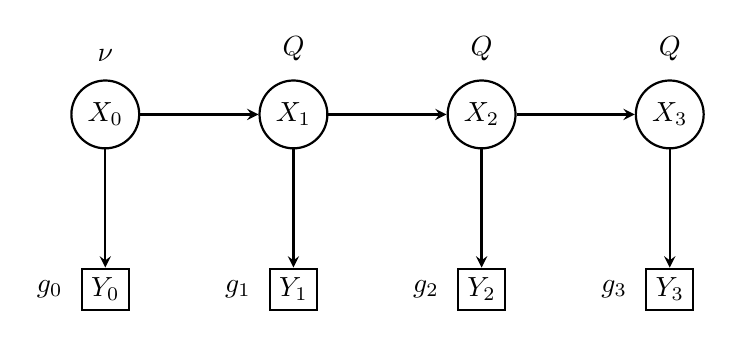
\begin{tikzpicture}[->,>=stealth,thick, node distance=1.5cm]

% Hidden states X_k
\node[draw,circle] (X0) {$X_0$};
\node[draw,circle, right=of X0] (X1) {$X_1$};
\node[draw,circle, right=of X1] (X2) {$X_2$};
\node[draw,circle, right=of X2] (X3) {$X_3$};

% Observations Y_k
\node[draw,rectangle, below=of X0] (Y0) {$Y_0$};
\node[draw,rectangle, below=of X1] (Y1) {$Y_1$};
\node[draw,rectangle, below=of X2] (Y2) {$Y_2$};
\node[draw,rectangle, below=of X3] (Y3) {$Y_3$};

% Arrows between hidden states (Markov transitions)
\draw (X0) -- (X1);
\draw (X1) -- (X2);
\draw (X2) -- (X3);

% Arrows from hidden states to observations (emissions)
\draw (X0) -- (Y0);
\draw (X1) -- (Y1);
\draw (X2) -- (Y2);
\draw (X3) -- (Y3);

% Optionally, label the transition and emission probabilities
\node[above=0.1cm of X0] {$\nu$};
\node[above=0.1cm of X1] {$Q$};
\node[above=0.1cm of X2] {$Q$};
\node[above=0.1cm of X3] {$Q$};

\node[left=0.1cm of Y0] {$g_0$};
\node[left=0.1cm of Y1] {$g_1$};
\node[left=0.1cm of Y2] {$g_2$};
\node[left=0.1cm of Y3] {$g_3$};

\end{tikzpicture}
\end{figure}

\begin{definition}[Hidden Markov Model]\label{def:HMM}
Let $(\mathsf{X},\mathcal{X})$ and $(\mathsf{Y},\mathcal{Y})$ be two measurable
spaces, and let $Q$ and $G$ denote, respectively, a Markov transition kernel on
$(\mathsf{X},\mathcal{X})$ and a transition kernel from $(\mathsf{X},\mathcal{X})$
to $(\mathsf{Y},\mathcal{Y})$. Define a Markov transition kernel $T$ on the
product space $(\mathsf{X}\times \mathsf{Y}, \mathcal{X}\otimes \mathcal{Y})$ as follows: for all bounded  measurable functions $f$, and all $(x,y) \in \mathsf{X}\times \mathsf{Y}$,
\begin{equation}\label{eq:HMM-kernel}
Tf(x,y) \;:=\; \int Q(x, \mathrm{d}x') \, G(x', \mathrm{d}y') f(x',y').
\end{equation}
Then, a Markov chain $\{(X_k,Y_k)\}_{k\ge 0}$ with transition kernel $T$ is called a \emph{hidden Markov model}.
\end{definition}
We may assume that there exists a probability measure $\lambda$ on $(\mathsf{Y},\mathcal{Y})$ such
that, for all $x \in \mathsf{X}$, $G(x, \cdot)$ is absolutely continuous with
respect to $\lambda$, i.e., $G(x, \cdot) \ll \lambda(\cdot)$,  with transition density function $g(x, \cdot)$. We also assume that there exists a probability
measure $\mu$ on $(\mathsf{X},\mathcal{X})$ such that 
for all $x \in \mathsf{X}$, $Q(x, \cdot) \ll \mu(\cdot)$ with transition
density function $q(x, \cdot)$.  The joint Markov
transition kernel $T$ is then dominated by the product measure $\mu \otimes \lambda$
and admits the transition density function
\[
t((x,y),(x',y')) \;:=\; q(x,x')\, g(x',y').
\]
\begin{proposition}\label{prop:conditional-independence-HMM}
Let $\{(X_k,Y_k)\}_{k\ge 0}$ be a Markov chain on the product space
$\mathsf{X}\times \mathsf{Y}$ with transition kernel $T$ defined by~\eqref{eq:HMM-kernel} and initial distribution $\nu(\rmd x)G(x,\rmd y)$. Then,
for any integer $p$, any ordered set of indices $k_1 < \cdots < k_p$, and any
bounded measurable functions $f_1,\dots,f_p$,
\begin{equation}\label{eq:HMM-cond-independence}
\mathbb{E}\Biggl[
\prod_{i=1}^{p} f_i(Y_{k_i}) \,\Big|\, X_{k_1}, \dots, X_{k_p} 
\Biggr]
\;=\; \prod_{i=1}^{p} \int_{\mathsf{Y}} f_i(y) \, G(X_{k_i}, \mathrm{d}y).
\end{equation}
\end{proposition}

\begin{proof}
For all bounded measurable function $h$, we have
\begin{align*}
\mathbb{E}\Biggl[ \prod_{i=1}^{p} f_i(Y_{k_i}) \, h(X_{k_1}, \dots, X_{k_p}) \Biggr]
&= \int \nu(\mathrm{d}x_0) G(x_0,\mathrm{d}y_0)
\prod_{i=1}^{k_p} Q(x_{i-1}, \mathrm{d}x_i) G(x_i, \mathrm{d}y_i) \\
&\quad \times \Biggl[ \prod_{i=1}^{p} f_i(y_{k_i}) \Biggr] \, h(x_{k_1},\dots,x_{k_p}) \\
&= \int \nu(\mathrm{d}x_0) \prod_{i=1}^{k_p} Q(x_{i-1},\mathrm{d}x_i) \, h(x_{k_1},\dots,x_{k_p}) \\
&\quad \times \prod_{i \notin \{k_1,\dots,k_p\}} \int_{\mathsf{Y}} G(x_i, \mathrm{d}y_i)
\prod_{i \in \{k_1,\dots,k_p\}} \int_{\mathsf{Y}} f_i(y_i) G(x_i, \mathrm{d}y_i),
\end{align*}
which completes the proof.
\end{proof}
The joint probability of the unobservable states and the observations up to
index $n$ is given as follows. For any bounded measurable function $f$,
\begin{multline}\label{eq:joint-probability-HMM}
\mathbb{E}\bigl[f(X_0, Y_0, \dots, X_n, Y_n)\bigr] =
\int f(x_0, y_0, \dots, x_n, y_n) \, 
\nu(\mathrm{d}x_0) g(x_0, y_0)
\\ \times \prod_{k=1}^{n} Q(x_{k-1}, \mathrm{d}x_k) g(x_k, y_k) \, \lambda^{\otimes (n+1)}(\mathrm{d}y_0, \dots, \mathrm{d}y_n),
\end{multline}
where $\lambda^{\otimes (n+1)}$ denotes the $(n+1)$-fold product measure on $(\mathsf{Y}^{n+1},\mathcal{Y}^{\otimes (n+1)})$. Marginalizing over the unobservable states $X_0, \dots, X_n$ yields the
distribution of the observations alone:
\begin{equation}\label{eq:marginal-observations}
\mathbb{E}\bigl[f(Y_0, \dots, Y_n)\bigr] =
 \int f(y_0, \dots, y_n) \, L_{n}(y_0, \dots, y_n) \, 
\lambda^{\otimes (n+1)}(\mathrm{d}y_0, \dots, \mathrm{d}y_n),
\end{equation}
where $L_{n}$ is defined below and plays a central role in likelihood-based inference.
\begin{definition}[Likelihood]\label{def:likelihood-HMM}
The \emph{likelihood} of the observations $(Y_0, \dots, Y_n)$ is the
probability density function with respect to $\lambda^{\otimes (n+1)}$, given, for all $ (y_0, \dots, y_n) \in \mathsf{Y}^{n+1}$, by
\begin{equation}\label{eq:likelihood-HMM}
L_{n}(y_0, \dots, y_n) :=
\int \nu(\mathrm{d}x_0) g(x_0, y_0) 
\prod_{k=1}^{n} Q(x_{k-1}, \mathrm{d}x_k) g(x_k, y_k).
\end{equation}
The \emph{log-likelihood function} is defined as
\begin{equation}\label{eq:log-likelihood-HMM}
\ell_{n} \;:=\; \log L_{n}.
\end{equation}
\end{definition}


\subsection{Sequential Monte Carlo methods for HMMs}
We now specialize the sampling techniques introduced above to hidden Markov
models (HMMs). As in previous chapters, we consider the HMM  where $Q$ denotes the Markov transition kernel of the hidden
chain, $\nu$ is the distribution of the initial state $X_0$, and $g(x,y)$, for
$x\in \mathsf{X}$ and $y \in \mathsf{Y}$, denotes the conditional density of the
observation given the state, with respect to the measure $\lambda$ on
$(\mathsf{Y},\mathcal{Y})$.  To simplify the notation, we will also use the shorthand
\[
g_k(\cdot) := g(\cdot, Y_k).
\] 
In the following we consider the following distributions.
\begin{itemize}
\item For all $0\leq k \leq n$, $\varphi_k$ is the conditional distribution of $X_k$ given $Y_{0:k}$, and is referred to as the filtering distribution at time $k$.
\item For all $0\leq k \leq \ell \leq n$, $\varphi_{k:\ell|n}$ is the conditional distribution of $X_{k:\ell}$ given $Y_{0:n}$, and is referred to as the joint smoothing  distribution of $X_{k:\ell}$ given $Y_{0:n}$.
\item  For all $0\leq k \leq n$, $\varphi_{k|n}\varphi_{k:k|n}$, is the marginal smoothing distribution at time $k$.
\end{itemize}
Note that for all bounded measurable functions $f$,
\[
\varphi_0(f) = \frac{\int f(x_0)\, g_0(x_0)\, \nu(\mathrm{d}x_0)}
{\int g_0(x_0)\, \nu(\mathrm{d}x_0)}.
\]
Therefore, $\varphi_0(f)$ can be estimated using self-normalized importance sampling. Sample $(\xi_0^1,\ldots,\xi_0^N)$ i.i.d. with probability density $\chi$ and associate each $\xi_0^i$ with $\omega_0^i = g_0(\xi^i_0)/\chi(\xi_0^i)$ and compute
$$
\varphi^N_0(f) = \sum_{i=1}^N\frac{\omega_0^i}{\sum_{j=1}^N\omega_0^j}f(\xi_0^i).
$$
In addition, for all $n\geq 0$ and all bounded measurable functions $f$,
$$
\varphi_{0:n|n}(f) =  \frac{\int \nu(x_0) g_0(x_0) 
\prod_{k=1}^{n} q(x_{k-1}, x_k) g_k(x_k)f(x_{0:n})\mu^{\otimes (n+1)}(\mathrm{d}x_0, \dots, \mathrm{d}x_n),}{\int \nu(x_0) g_0(x_0) 
\prod_{k=1}^{n} q(x_{k-1}, x_k) g_k(x_k)\mu^{\otimes (n+1)}(\mathrm{d}x_0, \dots, \mathrm{d}x_n)}.
$$
Therefore, it is straightforward to note that for all $0\leq k \leq n-1$,
\begin{align*}
\varphi_{0:k+1|k+1}(x_{0:k+1}) \propto \varphi_{0:k|k}(x_{0:k})q(x_{k}, x_{k+1})g_{k+1}(x_{k+1})
\end{align*}
Therefore,  for all bounded measurable functions $f$,
$$
\varphi_{k+1}(f) = \frac{\int \varphi_{k}(x_{k})q(x_{k}, x_{k+1})g_{k+1}(x_{k+1})f(x_{k+1})\mu(\rmd x_{k})\mu(\rmd x_{k+1})}{\int \varphi_{k}(x_{k})q(x_{k}, x_{k+1})g_{k+1}(x_{k+1})\mu(\rmd x_{k})\mu(\rmd x_{k+1})}.
$$
As these integrals are intractable, if at time $k$ we have access to a weighted sample $\{(\omega_k^i,\xi_k^i) \}_{1\leq i \leq N}$ we may estimate $\varphi_{k+1}$  by
\begin{align*}
\tilde\varphi^N_{k+1}(x_{k+1}) \propto \sum_{i=1}^N\omega_k^iq(\xi^i_{k}, x_{k+1})g_{k+1}(x_{k+1}).
\end{align*}
This approximation suggests that an importance sampling estimator of $\varphi_{k+1}(f) $ can be obtained as follows.
\begin{itemize}
\item For all $1\leq i \leq N$ sample $I_{k+1}^i$ in $\{1,\ldots, N\}$ with probabilities proportional to $\{\omega_k^i\}_{1\leq i \leq N}$.
\item For all $1\leq i \leq N$ sample $\xi_{k+1}^i \sim P(\xi_k^{I_{k+1}^i},\cdot)$ where $P$ is a proposal kernel.
\item For all $1\leq i \leq N$, compute
$$
\omega_{k+1}^i = \frac{q(\xi_k^{I_{k+1}^i}, \xi^i_{k+1})g_{k+1}(\xi^i_{k+1})}{p(\xi_k^{I_{k+1}^i},\xi_k^i)}.
$$
\end{itemize}
Then, $\varphi_{k+1}(f) $ is estimated by
$$
\varphi^N_{k+1}(f) = \sum_{i=1}^N\frac{\omega_{k+1}^i}{\sum_{j=1}^N\omega_{k+1}^j}f(\xi_{k+1}^i).
$$




\chapter{Variational inference and autoencoders}


\section{Evidence Lower Bound}
In this chapter, we consider models with latent (unobserved) data. Let $(Z,X)$ be random variables in $\mathbb{R}^d\times \mathbb{R}^m$. We assume that the law of $(Z,X)$ has a density $(z,x)\mapsto p(z,x)$ with respect to a reference measure. In this setting, we write
$$
(z,x)\mapsto p(z,x) = p(z)p(x|z)\,,
$$
where $z\mapsto p(z)$ is a prior density for $Z$ and $x \mapsto p(x|z)$ is the conditional density (likelihood) of $X$ given $Z$. We do not have access to the conditional density of $Z$ given $X$, since this density is given by:
$$
z\mapsto p(z|x) = \frac{p(z)p(x|z)}{p(x)}\propto p(z)p(x|z)\,, 
$$
where $p(x) = \int p(z)p(x|z) \mathrm{d} z$ is an intractable integral. The conditional law of latent variables given observations is of utmost importance in many machine learning approaches. For instance, in the E-step of the EM algorithm, the intermediate quantity requires to compute an expecation under such a distribution. In most situations, this distribution cannot be sampled from easily. Standard solutions to sample approximately from $p(z|x)$ include Markov Chain (or Sequential) Monte Carlo methods. In this chapter, we focus on variational approaches where $p(z|x)$ is replaced by a simpler distribution obtained by solving an optimization problem. 

\medskip

In variational inference, we introduce a variational family i.e. a family of densities to  approximate $z\mapsto p(z|x)$. Let $\mathcal{D}$ be such a family, where the densities $q \in\mathcal{D}$ satisfy the two following assumptions.
\begin{itemize}
\item For all $q\in \mathcal{D}$, $q$ is easy to evaluate.
\item For all $q\in \mathcal{D}$, $q$ is easy to sample from.
\end{itemize}

\medskip

Then, for all $x$ and all $q\in \mathcal{D}$, writing $\mathrm{KL}$ the Kullback-Leibler divergence between two probability distributions,
\begin{align*}
\mathrm{KL}\left(q\|p(\cdot|x)\right) = \int q(z) \log \frac{q(z)}{p(z|x)} \mathrm{d}z&= \mathbb{E}_{q}[\log q(Z)] - \mathbb{E}_{q}[\log p(Z|x)]\,,\\
 &= \mathbb{E}_{q}[\log q(Z)] - \mathbb{E}_{q}[\log p(Z,x)]+\log p(x)\,,\\
&= -\mathcal{L}_x(q)+\log p(x)\,,
\end{align*}
where
$$
\mathcal{L}_x(q) = \mathbb{E}_{q}\left[\log \frac{p(Z,x)}{q(Z)}\right]\,.
$$
Using Jensen's inequality, we obtain $\mathrm{KL}\left(q\|p(\cdot|x)\right) \geq 0$ so that
$$
\mathcal{L}_x(q)\leq \log p(x)\,.
$$
This inequality justifies the name Evidence Lower BOund for $\mathcal{L}_x = \mathbb{E}_{q}[\log (p(Z,x)/q(Z))]$. In variational inference, we then aim to approximate  $p(\cdot|x)$ by $q_{*}$ where:
$$
q_* \in \mathrm{argmax}_{q\in \mathcal{D}}\;\mathcal{L}_x(q)\,.
$$

\section{Coordinate ascent variational inference}
The most straightforward approach to solve the optimization problem is to consider a mean-field variational family  i.e. to choose $\mathcal{D}$ such that: 
$$
\mathcal{D} = \left\{z\mapsto q(z) = \prod_{j=1}^dq_j(z_j)\;;\; q_j \,\mbox{is\, a\, density} \right\}\,.
$$
Even when considering a simple variational family such as $\mathcal{D}$, it is not possible to maximize the ELBO explicitly. Assume therefore that we want to optimize $\mathrm{ELBO}(q) $ on $q_j$ only for some $1\leq j \leq d$, the other densities $(q_\ell)_{\ell\neq j}$ being kept fixed.
Write $z_{-j} = (z_\ell)_{1\leq \ell \leq d; \ell \neq j}$, and for all $q\in \mathcal{D}$,  $q_{-j}(z_{-j}) = \prod_{1\leq \ell \leq d; \ell \neq j}q_{\ell}(z_{\ell})$. Then,
\begin{align*}
\mathcal{L}_x(q) &= \int \left\{\prod_{\ell=1}^dq_\ell(z_\ell)\right\} \left\{\log (p(z_{-j},x)p(z_j|z_{-j},x)) - \sum_{\ell=1}^d\log q_\ell(z_\ell)\right\}\rmd z_1\ldots \rmd z_d\,,\\
&= \int q_j(z_j)\int \left\{\prod_{\ell=1, \ell\neq j}^dq_\ell(z_\ell)\right\} \left\{\log (p(z_{-j},x)p(z_j|z_{-j},x))\rmd z_{-j}\right\}\rmd z_j \\
&\hspace{3cm}- \sum_{\ell=1}^d\int q_\ell(z_\ell)\log q_\ell(z_\ell)\rmd z_\ell  \,\\
&= \mathbb{E}_{q_j}\left[\mathbb{E}_{q_{-j}}\left[\log p(Z_j | Z_{-j},x)\right]\right] - \mathbb{E}_{q_j}\left[\log q_j(Z_j)\right]  + \mathrm{C}
\end{align*}
%\begin{align*}
%\mathcal{L}_x(q) &= \mathbb{E}_{q}\left[\log \frac{p(Z_1,\ldots,Z_d,x)}{\prod_{j=1}^dq_j(Z_j)}\right]\,,\\
%&= \mathbb{E}_{q_j}\left[\mathbb{E}_{q_{-j}}\left[\log p(Z_j | Z_{-j},x)\right]\right] - \mathbb{E}_{q_j}\left[\log q_j(Z_j)\right]  + \mathrm{C}
%\end{align*}
where $\mathrm{C}$ does not depend on $q_j$. %,  $z_{-j} = (z_\ell)_{1\leq \ell \leq d; \ell \neq j}$ and $q_{-j}(z_{-j}) = \prod_{1\leq \ell \leq d; \ell \neq j}q_{\ell}(z_{\ell})$.  
Consider the density $\tilde q_j$ such that
$$
\tilde q_j(z_j) \propto \exp\left(\mathbb{E}_{q_{-j}}\left[\log p(z_j | Z_{-j},x)\right]\right)\,,
$$
i.e. the density given by $\tilde q_j(z_j)= \exp(\mathbb{E}_{q_{-j}}[\log p(z_j | Z_{-j},x)])/C_j$ where $C_j$ does not depend on $z_j$ ($C_j$ is the normalizing constant to obtain a density). Therefore,
$$
\mathcal{L}_x(q) = -\mathbb{E}_{q_j}\left[\log \frac{q_j(Z_j)}{\tilde q_j(Z_j) }\right]  + \mathrm{C} + \log C_j = -\mathrm{KL}(q_j\|\tilde q_j)  + \mathrm{C} + \log C_j\,.
$$
Therefore, optimizing  $\mathcal{L}_x(q) $ on $q_j$ only, the other densities $(q_\ell)_{\ell\neq j}$ being kept fixed, yields an optimum given by $\tilde q_j$.
The algorithm Coordinate Ascent Variational Inference (CAVI) proposes therefore to sequentially update  $q_j$, $1\leq j \leq d$ until a stopping criterion is met. In Algorithm~\ref{alg:CAVI}, we propose a version of the algorithm where the variational distribution of only one component of $Z$ is updated at each iteration, of course many alternatives can be considered. A standard alternative is to update each variational distribution at each iteration.

\begin{algorithm}[H] \label{alg:CAVI}
    \KwData{Observation $x$, initial variational distribution $\{q_j^{(0)}\}_{1\leq j \leq d}$, maximum number of iteration $N$}
    \KwResult{A variational distribution for each coordinate of $Z$, $q^{(N)}_j$, $1\leq j\leq d$.}
    \For {$ k= 1 \to N$}{
        Draw $j\in\{1,\ldots,d\}$ uniformly at random;

        Set $q^{(k)}_\ell = q^{(k-1)}_\ell$ for all $1\leq \ell \leq d$, $\ell \neq j$ and $q^{(k)}_{-j} = \prod_{1\leq \ell \leq d, \ell\neq j} q^{(k)}_{\ell}$;

        Set $$q^{(k)}_j(z_j) \propto \exp\left(\mathbb{E}_{q_{-j}^{(k)}}\left[\log p(z_j | Z_{-j},x)\right]\right)$$
;
}
\end{algorithm}

\section{Application to a mixture of Gaussian distributions}
This example can be found in  \cite{blei2017variational}. Consider a mixture of $K$ Gaussian distributions with means $\mu = (\mu_k)_{1\leqslant k \leqslant K}$ and variance 1. The variables  $\mu = (\mu_k)_{1\leqslant k \leqslant K}$ are  i.i.d. Gaussian with mean 0 and variance $\sigma^2$. For all $1\leq i\leq n$, we denote by $c_i\in\{1, \ldots, K\}$ the group the $i$-th observation belongs to. The variables $\mu$ and $c$ are not observed.  The random variables $c= (c_i)_{1\leq i\leq n}$ are independent of  $\mu$ and are independent with multinomial distribution with parameters $\{\omega_1,\ldots,\omega_K\}$, where $\sum_{k=1}^K\omega_k = 1$.  

Conditionally on  $\mu$ and $c$, the observations $(X_i)_{1\leqslant i\leqslant n}$ are independent and $X_i$ has a Gaussian distribution with mean $\mu_{c_i}$ and variance $1$. Marginalizing on $c$, conditionally on  $\mu$, the observations $(X_i)_{1\leqslant i\leqslant n}$ are i.i.d. and the conditional probability density of $X_1$ is:
$$
x\mapsto p(x|\mu) = \sum_{k=1}^K \omega_k \varphi_{\mu_k,1}(x)\,,
$$
where $\varphi_{\mu_k,\eta^2}$ the Gaussian probability density function with mean $\mu_k$ and  variance $\eta^2$. The joint likelihood is therefore:
$$
p(x_{1:n}) = \int p(x_{1:n}|\mu) p(\mu) \mathrm{d} \mu = \int \prod_{i=1}^n p(x_i|\mu) p(\mu) \mathrm{d} \mu = \int \prod_{i=1}^n \left(\sum_{k=1}^K \omega_k \varphi_{\mu_k,1}(x_i)\right) p(\mu) \mathrm{d} \mu\eqsp.
$$
Writing $z = (\mu,c)$, our objective is to estimate $p(\mu,c|x)$ where $c = (c_1,\cdots,c_n)$ are the components of the observations. Consider the following `mean-field` approximation:
$$
q(\mu,c) = \prod_{k=1}^K \varphi_{m_k,s_k}(\mu_k)\prod_{i=1}^n \mathrm{Cat}_{\phi_i}(c_i)\,, 
$$
which means that under $q$:
\begin{itemize}
\item $\mu$ and  $c$ are independent.
\item $(\mu_{k})_{1\leqslant k \leqslant K}$ are independent Gaussian random variables with means $(m_{k})_{1\leqslant k \leqslant K}$ and variances $(s_{k})_{1\leqslant k \leqslant K}$.
\item $(c_{i})_{1\leqslant i \leqslant n}$ are independent with  multinomial distributions with parameters  $(\phi_i)_{1\leqslant i \leqslant n}$.%: $q(c_i=k) = \phi_i(k)$ for $1\leqslant k \leqslant K$. 
\end{itemize}
Write $\mathcal{D}$ this family where the means $(m_{k})_{1\leqslant k \leqslant K}\in \mathbb{R}^K$, and variances $(s_{k})_{1\leqslant k \leqslant K}\in (\mathbb{R}_+^*)^K$ and the parameters  $(\phi_i)_{1\leqslant i \leqslant n}\in \mathbb{S}_K^n$ where $\mathbb{S}_K$ is the simplex of dimension $K$.  Then, we aim at solving the optimization problem:
$$
q^* = \mathrm{Argmin}_{q\in\mathcal{D}}\; \mathrm{KL}\left(q\|p(\cdot|x)\right)\,.
$$
Note that
\begin{align*}
\mathrm{KL}\left(q\|p(\cdot|x)\right) &= \mathbb{E}_q[\log q(\mu,c)] - \mathbb{E}_q[\log p(\mu,c|x)]\,,\\
 &= \mathbb{E}_q[\log q(\mu,c)] - \mathbb{E}_q[\log p(\mu,c,x)]+\log p(x)\,,\\
&= -\mathcal{L}_x(q)+\log p(x)\,,
\end{align*}
where
$$
\mathcal{L}_x(q)= -\mathbb{E}_q[\log q(\mu,c)] + \mathbb{E}_q[\log p(\mu,c,x)] \,.
$$
CAVI algorithm computes iteratively $1\leqslant k \leqslant K$,
$$
q(\mu_k) \propto \mathrm{exp}\left(\mathbb{E}_{\tilde q_{\mu_k}}[\log p(\mu_k|x,c,\mu_{-k})]\right)
$$
and for all $1\leqslant i \leqslant n$,
$$
q(c_i) \propto \mathrm{exp}\left(\mathbb{E}_{\tilde q_{c_i}}[\log p(c_i|x,c_{-i},\mu)]\right)\,,
$$
where $\mu_{-k} = (\mu_j)_{1\leq j \leq K, j\neq k}$, $c_{-i} = (c_j)_{1\leq j \leq n, j\neq i}$, and  $\mathbb{E}_{\tilde q_z}$ is the expectation under the variational distribution of all variables except $z$. 
%\begin{itemize}
%\item $\tilde p_i(c_i|x)$ is the conditional distribution of $c_i$ given the observations and the other parameters  and $\tilde p_k(\mu_k|x)$ is the conditional distribution of $\mu_k$ given the observations and the other parameters.
%\item $\mathbb{E}_{\tilde q_z}$ is the expectation under the variational distribution of all variables except $z$.
%\end{itemize}
\subsubsection*{Update of the variaitonal distribution of $c_i$, $1\leq i \leq n$}
Note that
$$
p(c_i|x,c_{-i},\mu) \propto p(c_i)p(x_i|c_i,\mu) \propto p(c_i)\prod_{k=1}^K \left(\varphi_{\mu_k,1}(x_i)\right)^{1_{c_i=k}}\,. 
$$
Then,
$$
\mathbb{E}_{\tilde q_{c_i}}[\log p(c_i|x,c_{-i},\mu)] = \log p(c_i) + \sum_{k=1}^K 1_{c_i=k} \mathbb{E}_{\tilde q_{c_i}}[\log \varphi_{\mu_k,1}(x_i)]
$$
and
\begin{align*}
\mathrm{exp}\left(\mathbb{E}_{\tilde q_{c_i}}[\log p(c_i|x,c_{-i},\mu)]\right) &\propto p(c_i) \mathrm{exp}\left(\sum_{k=1}^K 1_{c_i=k} \mathbb{E}_{\tilde q_{c_i}}[\log \varphi_{\mu_k,1}(x_i)]\right)\,\\
&\propto p(c_i) \mathrm{exp}\left(\sum_{k=1}^K 1_{c_i=k} \mathbb{E}_{\tilde q_{c_i}}[-(x_i-\mu_k)^2/2]\right)\,.
\end{align*}
The update writes:
$$
\phi_i(k) \propto \omega_k\mathrm{exp}\left(m_k x_i - \frac{m^2_k + s_k}{2}\right)\,.
$$

\subsubsection*{Update of the variaitonal distribution of $\mu_k$, $1\leq k \leq K$}
On the other hand,
$$
p(\mu_k|x,c,\mu_{-k}) \propto p(\mu_k)\prod_{i=1}^np(x_i|c_i,\mu) \,. 
$$
Then,
$$
\mathbb{E}_{\tilde q_{\mu_k}}[\log p(\mu_k|x,c,\mu_{-k})] = \log p(\mu_k) + \sum_{i=1}^n \mathbb{E}_{\tilde q_{\mu_k}}[\log p(x_i|\mu,c_i)]
$$
and
\begin{align*}
\mathrm{exp}\left(\mathbb{E}_{\tilde q_{\mu_k}}[\log p(\mu_k|x,c,\mu_{-k})]\right) &\propto p(\mu_k) \mathrm{exp}\left(\sum_{i=1}^n\sum_{\ell=1}^K  \mathbb{E}_{\tilde q_{\mu_k}}[1_{c_i=\ell}\log \varphi_{\mu_\ell,1}(x_i)]\right)\,\\
&\propto p(\mu_k) \mathrm{exp}\left(\sum_{i=1}^n \phi_i(k) \mathbb{E}_{\tilde q_{\mu_k}}[\log \varphi_{\mu_k,1}(x_i)]\right)\,\\
&\propto \mathrm{exp}\left(-\frac{\mu_k^2}{2\sigma^2}-\frac{1}{2}\sum_{i=1}^n \phi_i(k)(x_i-\mu_k)^2\right)\,,\\
&\propto \mathrm{exp}\left(-\frac{\mu_k^2}{2\sigma^2}+\sum_{i=1}^n \phi_i(k)x_i\mu_k - \frac{1}{2}\sum_{i=1}^n \phi_i(k)\mu^2_k\right)\,.
\end{align*}
The update writes therefore,
$$
m_k = \frac{\sum_{i=1}^n \phi_i(k)x_i}{1/\sigma^2 + \sum_{i=1}^n \phi_i(k)}\quad\mathrm{and}\quad s_k = \frac{1}{1/\sigma^2 + \sum_{i=1}^n \phi_i(k)}\,. 
$$

\begin{algorithm}[H] \label{alg:CAVI:mixtureGauss}
    \KwData{Observations $x= (x_1,\ldots,x_n)$, initial values of $\phi_i(k)$, $m_k$ and $s_k$, $1\leq k \leq K$, $1\leq i \leq n$, maximum number of iteration $N$}
    \KwResult{A variational distribution for each coordinate of $\mu_k$ and  $c_i$, $1\leq k\leq K$, $1\leq i\leq n$.}
    \For {$ p= 1 \to N$}{
    
\For{$i = 1 \to n$}{
Set $$
\phi_i(k) \propto \omega_k\mathrm{exp}\left(m_k x_i - \frac{m^2_k + s_k}{2}\right)\,.
$$;
}

\For{$k = 1 \to K$}{
Set 
$$
m_k = \frac{\sum_{i=1}^n \phi_i(k)x_i}{1/\sigma^2 + \sum_{i=1}^n \phi_i(k)}\quad\mathrm{and}\quad s_k = \frac{1}{1/\sigma^2 + \sum_{i=1}^n \phi_i(k)}\,. 
$$;
}
    
}
\caption{A version of CAVI algorithm for a Bayesian mixture of Gaussian distributions.}
\end{algorithm}

\section{Variational Autoencoders}
Variational Auto-Encoders (VAE) are very popular approaches to introduce approximations of a target conditional distribution in the context of latent data models. Assume that $(X_1,\ldots,X_n)$ are i.i.d. random variables in $\mathsf{X}$ with unknown probability distribution function $\pi_{\mathrm{data}}$. We consider a family of joint probability distributions $\{(z,x) \mapsto  p_{\theta}(z,x)\}_{\theta\in\Theta}$ on $(\mathsf{Z}\times \mathsf{X}, \mathcal{Z}\times \mathcal{X})$ where $Z$ is a latent variable and $X$ is the observation. In this setting, we often write, for all $\theta\in\Theta$, $x\in\mathsf{X}$, $z\in\mathsf{Z}$,
$$
p_{\theta}(z,x) = p_{\theta}(z)p_{\theta}(x|z)\eqsp.
$$
The latent variable generative model defines a joint density $(z,x)\mapsto p_\theta(x, z)$  on $(\mathsf{Z}\times \mathsf{X}, \mathcal{Z}\times \mathcal{X})$  by specifying a prior $z\mapsto p_{\theta}(z)$ over the latent variable $Z$ and a conditional density $x\mapsto p_\theta(x|z)$ also referred to as the decoder.  The normalized loglikelihood is therefore given by
$$
\ell_n(\theta) = \frac{1}{n}\sum_{i=1}^n \log p_{\theta}(X_i) = \frac{1}{n}\sum_{i=1}^n \log \int p_{\theta}(z)p_{\theta}(X_i|z)\rmd z\eqsp,
$$
and the conditional distribution $p_{\theta}(z|x)\propto p_{\theta}(z)p_{\theta}(x|z)$. In most cases, maximizing the average
marginal log-likelihood of the data is not possible, as the marginal likelihood functions $p_{\theta}(X_i)$, $1\leqslant i \leqslant n$, are not vailable explicitly as the integral for marginalizing the latent variable is intractable.  Since a maximum likelihood estimator cannot be computed simply, VAEs introduce a variational approach wich aims at simultaneously providing a parameter estimate  and an approximation of the conditional distribution of the latent variable given the observation.  Consider a family of probability density functions $\{(z,x) \mapsto q_{\varphi}(z|x)\}_{\varphi\in\Phi}$. Then, we can write, for all $\varphi\in\Phi,\theta\in\Theta$, $x\in\mathsf{X}$,
\begin{align*}
\log p_\theta(x) = \int \log p_\theta(x) q_{\varphi}(z|x) \rmd z &= \mathbb{E}_{q_{\varphi}(\cdot|x)}\left[\log p_\theta(x)\right] \\
&= \mathbb{E}_{q_{\varphi}(\cdot|x)}\left[\log \frac{p_\theta(Z,x)}{p_\theta(Z|x)}\right] \\
&= \mathbb{E}_{q_{\varphi}(\cdot|x)}\left[\log \frac{q_{\varphi}(Z|x)}{p_\theta(Z|x)}\right]  + \mathbb{E}_{q_{\varphi}(\cdot|x)}\left[\log \frac{p_\theta(Z,x)}{q_{\varphi}(Z|x)}\right] .
\end{align*}
The first term of the right-hand-side is the Kullback-Leibler divergence between $q_{\varphi}(\cdot|x)$ and $p_\theta(\cdot|x)$, so that $\log p_\theta(x)\geq \mathcal{L}(\theta,\varphi,x)$, where
$$
\mathcal{L}(\theta,\varphi,x) = \mathbb{E}_{q_{\varphi}(\cdot|x)}\left[\log \frac{p_\theta(Z,x)}{q_{\varphi}(Z|x)}\right]
$$
is the Evidence Lower BOund (ELBO). 
%In order to approximate $z\mapsto p_\theta(z|x)$, VAE propose to solve the optimization problem:
%$$
%\widehat \varphi \in \mathrm{argmin}_{\varphi\in\Phi} \mathcal{L}(\theta,\varphi,x)\eqsp.
%$$
This motivates the introduction of the following loss function:
$$
\mathcal{L}(\theta,\varphi) = \mathbb{E}_{\pi_{\mathrm{data}}}[-\mathcal{L}(\theta,\varphi,X)] = \mathbb{E}_{\pi_{\mathrm{data}}}\left[\mathbb{E}_{q_{\varphi}(\cdot|X)}\left[\log \frac{q_{\varphi}(Z|X)}{p_\theta(Z,X)}\right]\right]\eqsp.
$$
The empirical loss is then given by
$$
\mathcal{L}_n(\theta,\varphi) = \frac{1}{n}\sum_{i=1}^n\mathbb{E}_{q_{\varphi}(\cdot|X_i)}\left[\log \frac{q_{\varphi}(Z|X_i)}{p_\theta(Z,X_i)}\right]\eqsp,
$$
where $(X_1,\ldots,X_n)$ are i.i.d. with distribution $\pi_{\mathrm{data}}$, and we aim at solving the optimization problem:
\begin{equation}
\label{eq:optim:ELBO}
(\widehat \theta_n,\widehat \varphi_n) \in \mathrm{Argmax}_{\theta\in\Theta,\varphi\in\Phi}\eqsp \mathcal{L}_n(\theta,\varphi) \eqsp.
\end{equation}
The joint optimization of $\theta$ and $\varphi$ is a complex problem both for practical and theoretical reasons and many research works have been devoted to this problem in the past few years. In most cases, $\mathcal{L}_n(\theta,\varphi)$ cannot be computed explicitly since expectations under the variational distribution are not explicit. Therefore, $\mathcal{L}_n(\theta,\varphi) $ is replaced by a Monte Carlo estimate $\widehat{\mathcal{L}}_n(\theta,\varphi)$:
$$
\widehat{\mathcal{L}}_n(\theta,\varphi) =  \frac{1}{n}\sum_{i=1}^n\frac{1}{M}\sum_{j=1}^M\log \frac{q_{\varphi}(Z_{i,j}|X_i)}{p_\theta(Z_{i,j},X_i)}\eqsp,
$$ 
where for all $1\leqslant i \leqslant n$, $(Z_{i,1},\ldots,Z_{i,M})_{1\leqslant j\leqslant M}$ are i.i.d. with distribution $q_{\varphi}(\cdot|X_i)$.
\begin{figure}
\centering
\includegraphics[scale=0.9]{vae.png}
\caption{An illustration of a VAE. From "An Introduction to Variational Autoencoders", Kingma et al., 2019.}
\label{fig:vae}
\end{figure}



\appendix 

\chapter{M-estimation Z-estimation, maximum likelihood}

\section{Method of moments}
Consider a measurable space $(\Omega,\mathcal{F})$ and i.i.d. random variables $(X_1,\ldots,X_n)$ taking values in a measurable space $(\Xset,\Xsigma)$. We assume that we have access to probabilities $(\mathbb{P}_\theta)_{\theta\in\Theta}$, where $\Theta \subset\rset^d$. For all $\theta\in\Theta$, we write $\mathbb{E}_\theta$ the expectation under $\mathbb{P}_\theta$ and $\mathbb{V}_\theta$ the variance. The objective is to estimate the unknown parameter $\theta\in\Theta$. The method of moments consists in choosing $d$ functions $T_j:\Xset\to \rset$, $1\leq j\leq d$, such that $\mathbb{E}_\theta[|T_j(X_1)|]<\infty$. Then, write for all $1\leq j \leq d$, $\theta\in\Theta$,
$$
e_j(\theta) = \mathbb{E}_\theta[T_j(X_1)]\eqsp.
$$
As the quantities $e_j(\theta)$, $1\leq j \leq d$, $\theta\in\Theta$,  are usually unknown, they may be estimated by using empirical estimates. Assuming that for $1\leq j\leq d$, $\mathbb{E}_\theta[|T_j(X_1)|^2]<\infty$, the Bienayme-Tchebychev inequality allows to quantify the empirical estimation error: for all $\varepsilon>0$,
$$
\mathbb{P}_\theta\left(\left|\frac{1}{n}\sum_{i=1}^{n}T_j(X_i)-e_j(\theta)\right|\geq \varepsilon\right) \leq \frac{\mathbb{V}_\theta[T_j(X_1)]}{n\varepsilon^2}\eqsp.
$$
In order to estimate the unknown parameter $\theta$ we may consider the system of equations:
$$
\forall j\in\{1,\ldots,d\},\quad e_j(\theta) = \frac{1}{n}\sum_{i=1}^n T_j(X_i)\eqsp.
$$
Assuming that this system has a unique solution $\widehat \theta_n$, $\widehat \theta_n$ is referred to as the moment estimator associated with $\{T_j\}_{1\leq j\leq d}$.

\begin{example}
Let $(X_1,\ldots,X_n)$ be i.i.d. random variables with exponential distribution with parameter $\theta>0$. Using $T_1:x\mapsto x$ and $T_2:x\mapsto x^2$ we have for all $\theta>0$,
$$
e_1(\theta) = \theta^{-1}\quad\mathrm{and}\quad e_2(\theta) = 2\theta^{-2}\eqsp.
$$
The moment estimator associated with $T_1$ is
$$
\widehat \theta_{n,1} = \frac{n}{\sum_{i=1}^nX_i}\eqsp.
$$
The moment estimator associated with $T_2$ is
$$
\widehat \theta_{n,2} = \left(\frac{2n}{\sum_{i=1}^nX^2_i}\right)^{1/2}\eqsp.
$$
\end{example}

\section{Z-estimation}
The moment estimator associated with $\{T_j\}_{1\leq j\leq d}$ is a solution to a system of equations of the form
$$
\frac{1}{n}\sum_{i=1}^n\psi(\theta,X_i) = 0\eqsp,
$$
where for all $\theta\in\Theta$, $x\in\Xset$,
$$
\psi(\theta,x)  =\begin{pmatrix}T_1(x) - \mathbb{E}_{\theta}[T_1(X_1)]\\ \vdots \\T_d(x) - \mathbb{E}_{\theta}[T_d(X_1)]\end{pmatrix}\eqsp.
$$
Consider now arbitrary functions $\psi_j$, $1\leq j\leq d$, such that for all $\theta_*\in\Theta$, $1\leq j \leq d$, $\mathbb{E}_{\theta_*}[|\psi_j(\theta_*,X_1)|]<\infty$. A Z-estimator associated with $\psi = (\psi_1,\ldots,\psi_d)^\top$ is any solution $\widehat\theta_n$ satisfying
$$
\psi_n(\widehat\theta_n) = 0\eqsp,
$$
where for all $\theta\in\Theta$,
$$
\psi_n(\theta) = \frac{1}{n}\sum_{i=1}^n\psi(\theta,X_i)\eqsp.
$$
\begin{example}
Let $F$ be a distribution function on $\mathbb{R}$ such that for all $x\in\mathbb{R}$, $F(x) = 1 - F(-x)$. Let $(X_1,\ldots,X_n)$ be i.i.d with distribution function $F_{\theta_*}$ where for all $\theta\in\mathbb{R}$, $x\in\mathbb{R}$, $F_\theta(x) = F(x-\theta)$. In this setting,
$$
\mathbb{E}_\theta[X_1] = \theta\eqsp,
$$
which suggests to choose $\psi(\theta,x) = x-\theta$. In this case, the Z-estimator associated with $\psi$ is given by $\widehat\theta_n = n^{-1}\sum_{i=1}^nX_i$.
\end{example}


\section{Maximum likelihood}
\begin{definition}
Let $(\Xset,\Xsigma)$ be a measurable space equipped with a sigma-finite measure $\mu$. Let $(f_\theta)_{\theta\in\Theta}$ be a family of probability densities with respect to $\mu$ and $(X_i)_{1\leq i\leq n}$ be i.i.d. random variables with probability density $f_{\theta_*}$, $\theta_*\in\Theta$. The likelihood of $(X_i)_{1\leq i\leq n}$ is the function
$$
L_n:\theta\mapsto \prod_{i=1}^nf_\theta(X_i)\eqsp.
$$
A maximum likelihood estimator associated with $L_n$ is any estimator solution to the following optimization problem
$$
\widehat\theta_n\in \mathrm{Argmax}_{\theta\in\Theta} L_n(\theta)\eqsp.
$$
\end{definition}

\begin{example}
Let $(X_i)_{1\leq i\leq n}$ be i.i.d. Bernoulli random variables with parameter $\theta_*\in(0,1)$. For all $\theta\in(0,1)$,
$$
L_n(\theta) = \prod_{i=1}^n \theta^{X_i}(1-\theta)^{1-X_i}
$$
and
$$
\ell_n(\theta) = \log L_n(\theta) = \left(\sum_{i=1}^nX_i\right)\log\theta + \left(\sum_{i=1}^n(1-X_i)\right)\log(1-\theta)\eqsp.
$$
The function $\ell_n/n$ is stricly concave on $(0,1)$ with $\lim_{\theta\to 0}\ell_n(\theta)/n  =-\infty$ and $\lim_{\theta\to 1}\ell_n(\theta)/n =-\infty$. This function has therefore a unique maximum given by
$$
\widehat\theta_n = \frac{1}{n}\sum_{i=1}^nX_i\eqsp.
$$
\end{example}

\section{M-estimation}
Maximum likelihood estimators are defined as solutions to optimization problems. This is the case of many estimation procedures. Consider for instance a function $m:\Theta\times \Xset \to \mathbb{R}$, $(\theta,x)\mapsto m_\theta(x)$, such that for all $\theta,\theta_*\in\Theta$, $\mathbb{E}_{\theta_*}[|m_\theta(X_1)|]<\infty$ and consider also $M_n:\theta\mapsto n^{-1}\sum_{i=1}^n m_\theta(X_i)$. For all $\delta>0$,
$$
\mathbb{P}_{\theta_*}\left(\left|M_n(\theta) - M_{\theta_*}(\theta)\right|\geq \delta\right)\leq \frac{\mathbb{V}_{\theta_*}[m_\theta(X_1)]}{n\delta^2}\eqsp,
$$
where
$$
M_{\theta_*}(\theta) = \mathbb{E}_{\theta_*}[m_\theta(X_1)]\eqsp.
$$
A M-estimator is any solution to the following optimization problem:
$$
\widehat\theta_n\in \mathrm{Argmax}_{\theta\in\Theta} M_n(\theta)\eqsp.
$$

\begin{example}
For all $1\leq k\leq n$, let $x_k\in\mathbb{R}^d$ and consider $(\xi_k)_{1\leq k\leq n}$  i.i.d. random variables with distribution $\mathcal{N}(0,1)$ and the linear regression model:
$$
Y_k = \sum_{\ell=0}^{p}\beta_\ell \varphi_\ell(x_k) + \sigma\varepsilon_k\eqsp,
$$
where $\theta = (\sigma,\beta)\in\mathbb{R}_+^*\times \mathbb{R}^{p+1}$. The joint density of the observations is:
$$
f_n:\theta\mapsto (2\pi\sigma^2)^{-n/2}\mathrm{exp}\left(-\frac{1}{2\sigma^2}\sum_{k=1}^n\left(Y_k-\sum_{\ell=0}^{p}\beta_\ell \varphi_\ell(x_k)\right)^2\right)\eqsp.
$$
The maximum likelihood estimator of $\beta$ coincides with the mean squared error estimator
$$
\widehat{\beta}_n \in\mathrm{Argmin}_{\beta\in \mathbb{R}^{p+1}} \sum_{k=1}^n\left(Y_k-\sum_{\ell=0}^{p}\beta_\ell \varphi_\ell(x_k)\right)^2\eqsp.
$$
Consider the matrix $\Phi$ in $\mathbb{R}^{n\times(p+1)}$ such that for all $1\leq i \leq n$, $1\leq j \leq p+1$, $\Phi_{i,j} = \varphi_{j-1}(x_i)$. Then, $\widehat{\beta}_n$ is solution to 
$$
\Phi\Phi^\top \widehat{\beta}_n = \Phi Y\eqsp,
$$
where $Y = (Y_1,\ldots,Y_n)^\top$.
\end{example}

\section{Consistency}

%\subsection*{M-estimation}
When for all $\theta,\theta_*$, $\mathbb{E}_{\theta_*}[|m_\theta(X_1)|]<\infty$, by the law of large numbers, in $\mathbb{P}_{\theta_*}$-probability,
$$
M_n(\theta) = \frac{1}{n}\sum_{i=1}^nm_\theta(X_i) \rightarrow_{n\to\infty} M_{\theta_*}(\theta) = \mathbb{E}_{\theta_*}[m_\theta(X_1)]\eqsp.
$$
We also assume that $\theta_*$ is a maximum of $M_{\theta_*}$.
\begin{theorem}
Consider the following assumptions.
\begin{itemize}
\item For all $\theta_*\in\Theta$, in  $\mathbb{P}_{\theta_*}$-probability, $\mathrm{sup}_{\theta\in\Theta}|M_n(\theta)-M_{\theta_*}(\theta)|\to_{n\to \infty} 0$.
\item For all $\theta_*\in\Theta$ and $\varepsilon>0$,
$$
\mathrm{sup}_{\theta\in\Theta; |\theta-\theta_*|>\varepsilon}M_{\theta_*}(\theta)<M_{\theta_*}(\theta_*)\eqsp.
$$
\item $(\widehat \theta_n)_{n\geq 0}$ is such that there exists $(\rho_n)_{n\geq 0}$ satisfying for all $\theta_*\in\Theta$,  in  $\mathbb{P}_{\theta_*}$-probability, $\rho_n \to_{n\to \infty} 0$ and
$$
\mathrm{liminf}_{n\to \infty} \mathbb{P}_{\theta_*}\left(M_n(\widehat \theta_n)\geq M_n(\theta_*) -\rho_n\right) =1\eqsp.
$$
Then, for all $\theta_*\in\Theta$,  in  $\mathbb{P}_{\theta_*}$-probability, $\widehat \theta_n \to \theta_*$.
\end{itemize}
\end{theorem}

\begin{proof}
For all $\theta_*\in\Theta$, since $\theta_*$ is a maximum of $M_{\theta_*}$,
\begin{align*}
0\leq M_{\theta_*}(\theta_*) - M_{\theta_*}(\widehat\theta_n)&\leq  M_{\theta_*}(\theta_*) - M_n(\theta_*) + M_n(\theta_*) - M_n(\widehat\theta_n) + M_n(\widehat\theta_n) - M_{\theta_*}(\widehat\theta_n)\\
&\leq 2 \mathrm{sup}_{\theta\in\Theta}|M_n(\theta)-M_{\theta_*}(\theta)|+ \rho_n \\
&\hspace{3cm} + \left\{M_n(\theta_*)-M_n(\widehat \theta_n)-\rho_n\right\}\mathds{1}_{M_n(\theta_*) - \rho_n>M_n(\widehat \theta_n)}\eqsp.
\end{align*}
Let $\varepsilon>0$. There exists $\eta>0$ such that $M_{\theta_*}(\theta)\leq M_{\theta_*}(\theta_*)-\eta$ for all $\theta\in\Theta$ such that $|\theta-\theta_*|\geq \varepsilon$. Therefore, $\{|\widehat\theta_n-\theta_*|\geq \varepsilon\}\subset\{M_{\theta_*}(\widehat\theta_n)\leq M_{\theta_*}(\theta_*)-\eta\}$. This yields 
$$
\mathbb{P}_{\theta_*}\left(|\widehat\theta_n-\theta_*|\geq \varepsilon\right)\leq \mathbb{P}_{\theta_*}\left(M_{\theta_*}(\widehat\theta_n)\leq M_{\theta_*}(\theta_*)-\eta\right) \leq \mathbb{P}_{\theta_*}\left(M_{\theta_*}(\theta_*) - M_{\theta_*}(\widehat\theta_n)>\eta\right) \eqsp,
$$
which concludes the proof.
\end{proof}

\begin{remark}
If $\Theta$ is compact in $\mathbb{R}^d$, $M_{\theta_*}$ is continuous, and for all $\theta\neq\theta_*$, $M_{\theta_*}(\theta)<M_{\theta_*}(\theta_*)$, the second assumption is satisfied.
\end{remark}

%\subsection*{Z-estimation}
\subsection*{Exponential models}
Let $(X_1,\ldots,X_n)$ be i.i.d. random variables with density $p_{\theta_*}$ with respect to a reference measure $\mu$ on $(\mathbb{R}^d,\mathcal{B}(\mathbb{R}^d))$. The family $\{p_\theta\}_{\theta\in\Theta}$ is said to be in the exponential family if there exist $\eta:\theta\to \mathbb{R}^d$, $T:\Xset\to\mathbb{R}^d$, $h:\Xset\to\mathbb{R}_+$, $B:\Theta\to\mathbb{R}$ such that for all $x\in\Xset$,
$$
p_\theta(x) = h(x)\exp\left(\langle \eta(\theta);T(x)\rangle - B(\theta)\right)\eqsp.
$$

\begin{example}
\begin{itemize}
\item The density of a Poisson distribution with parameter $\theta>0$ is given by
$$
p_\theta:x \mapsto \frac{\theta^x}{x!} \rme^{-\theta}\eqsp,
$$
so that $h(x) = (x!)^{-1}$, $T(x)=x$, $\eta(\theta) = \log \theta$, $B(\theta) = -\theta$.
\item If $\theta = (\mu,\sigma^2)\in\mathbb{R}\times\mathbb{R}_+^*$ and $p_\theta$ is the Gaussian probability density with mean $\mu$ and variance $\sigma^2$, $h(x) = 1$, $T(x)=(x,x^2)^\top$, $\eta(\theta) = (\mu/\sigma^2,-1/(2\sigma^2))^\top$, $B(\theta) = \log(2\pi\sigma^2)/2 + \mu/(2\sigma^2)$.
\end{itemize}
\end{example}
The canonical exponential family is given, for all $x\in\Xset$, by 
$$
p_\eta(x) = h(x)\exp\left(\langle \eta;T(x)\rangle - A(\eta)\right)\eqsp,
$$
where
$$
A(\eta) = \log\left(\int h(x)\exp\left(\langle \eta;T(x)\rangle \right)\mu(\rmd x)\right)\eqsp.
$$

\bibliographystyle{apalike}
\bibliography{csbib}

%\printindex
\end{document}
